\documentclass[xcolor=dvipsnames,10pt,aspectratio=169]{beamer}
%\usetheme[hideallsubsections]{Hannover}
\usetheme[width=1.9cm]{Hannover} % plenty of themes to pick from
\usefonttheme[onlymath]{serif}
\graphicspath{{../../images/}}
\usepackage[utf8]{inputenc}
\usepackage[T1]{fontenc}
\usepackage{caption}
\usepackage{amsmath}
\usepackage{amsfonts}
\usepackage{amssymb}
\usepackage{braket}
\usepackage{bm}
\usepackage{textpos}
\usepackage{multicol}
\usepackage{graphicx,hyperref,url}
\usepackage{tikz}
\usepackage{verbatim}
\usepackage{pgfplots}
\usetikzlibrary{arrows,shapes}
\usecolortheme{crane} % plenty of color themes to pick from
\useinnertheme{rectangles}

\definecolor{UBCgreen}{RGB}{30, 77, 43} % UBC Blue (primary)
\definecolor{UBCgold}{RGB}{200, 195, 114} % UBC Grey (secondary)

\setbeamercolor{palette primary}{bg=UBCgreen,fg=white}
\setbeamercolor{palette secondary}{bg=UBCgreen,fg=white}
\setbeamercolor{palette tertiary}{bg=UBCgreen,fg=white}
\setbeamercolor{palette quaternary}{bg=UBCgreen,fg=white}
\setbeamercolor{palette sidebar primary}{fg=black,bg=UBCgold}
\setbeamercolor{palette sidebar secondary}{fg=black,bg=UBCgold}
\setbeamercolor{palette sidebar tertiary}{fg=black,bg=UBCgold}
\setbeamercolor{palette sidebar quaternary}{fg=black,bg=UBCgold}
\setbeamercolor{structure}{fg=UBCgreen} % itemize, enumerate, etc
\setbeamercolor{section in toc}{fg=UBCgreen} % TOC sections
\setbeamercolor{subsection in head/foot}{bg=UBCgold,fg=white}
\setbeamercolor{section in sidebar}{fg=UBCgreen}
\setbeamercolor{section in sidebar}{fg=UBCgreen}
\setbeamerfont{section in sidebar}{size=\small}
\setbeamerfont{subsection in sidebar}{size=\scriptsize}
\setbeamerfont{title in sidebar}{size=\tiny}
\setbeamerfont{author in sidebar}{size=\tiny}
\setbeamertemplate{page number in head/foot}[appendixframenumber]
\setbeamertemplate{navigation symbols}{\footnotesize\usebeamertemplate{page number in head/foot}}
\setbeamertemplate{frametitle}[default][left,colsep=-4bp,rounded=false]
\setbeamertemplate{section in toc}[bullets]

\addtobeamertemplate{title page}{}{%
    \begin{textblock*}{100mm}(0.445\textwidth,-22.4em)
      
\includegraphics[width=1.5cm]{./figures/CSU-Ram-357-617.png}
    \end{textblock*}
    \begin{textblock*}{85em}(-1.0em,-12em)
      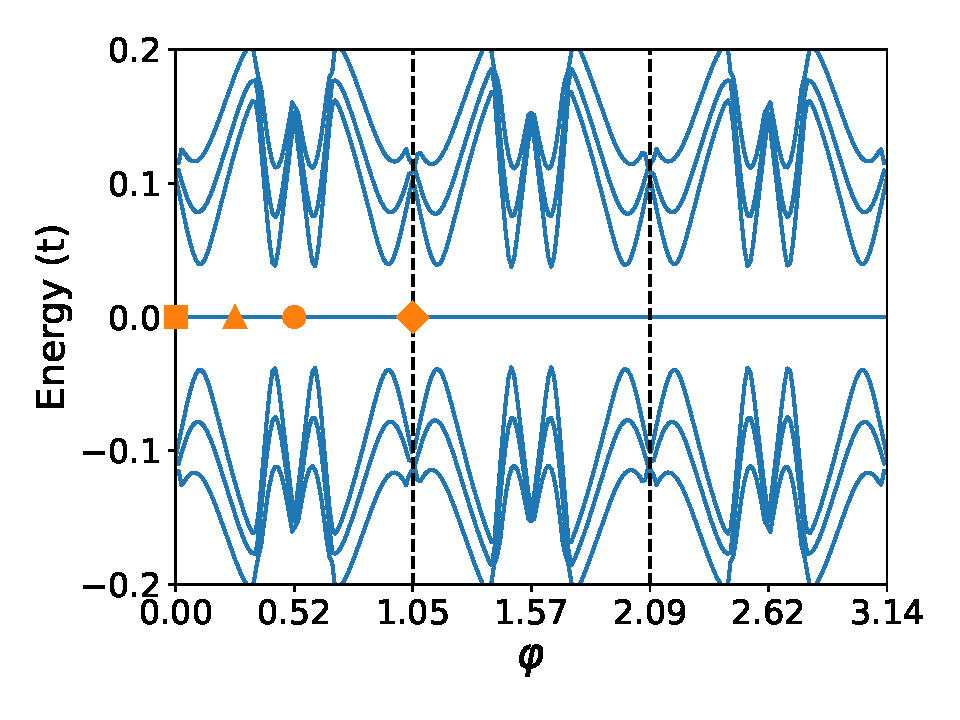
\includegraphics[width=0.18\textwidth]{./figures/spectral-flow-rotation-constant-vector-nr-50-w-1-mu-1_1.pdf}
    \end{textblock*}
    \begin{textblock*}{75em}(24.0em,-12em)
      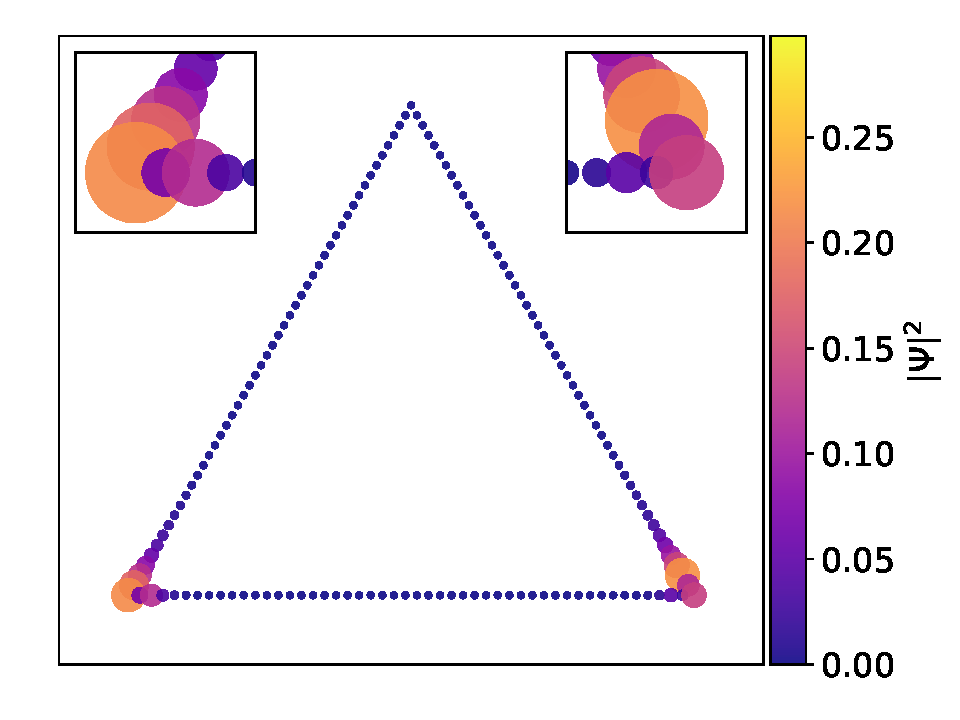
\includegraphics[width=0.19\textwidth]{./figures/GS-T-Square.pdf}
    \end{textblock*}
    \begin{textblock*}{100em}(-4.8em,16em)
      \tiny Powered by \LaTeX
    \end{textblock*}
}

\addtobeamertemplate{frametitle}{}{%
    \begin{textblock*}{100mm}(0.95\textwidth,-0.95cm)
      
\includegraphics[width=0.925cm]{./figures/CSU-Ram-357-617.png}
    \end{textblock*}
}
\makeatletter
\setbeamertemplate{sidebar canvas \beamer@sidebarside}%
                  [vertical shading][top=UBCgold,bottom=UBCgold]
\makeatother

%\addtobeamertemplate{sidebar left}{}{
%  \hspace{0.3cm}
%  \vspace{0.2cm}
%  
\includegraphics[align = l, width = 1cm]{./figures/CSU-Ram-357-617.png}
%}

%\setbeamertemplate{section in toc}{\hspace*{0em}\inserttocsection}
%\setbeamertemplate{subsection in toc}{\hspace*{2em}\inserttocsubsection}

\let\oldhat\hat
\renewcommand{\hat}[1]{\oldhat{\mathbf{#1}}}
\renewcommand{\vec}[1]{\mathbf{#1}}

\newcommand{\ham}{\mathcal{H}}
\newcommand{\ke}{k_{\epsilon}}
\newcommand{\kpm}{k_{\pm}}
\newcommand{\sx}{\sigma_x}
\newcommand{\sy}{\sigma_y}
\newcommand{\sz}{\sigma_z}
\newcommand{\so}{\sigma_0}
\newcommand{\cc}{c^{\dagger}}
\newcommand{\de}{\Delta}

\newcommand{\TT}{Emergent Topological Phenomena in Low-D Systems Induced by Gauge Potentials}
\newcommand{\ST}{Emergent topological phenomena in low-D systems induced by gauge potentials}
\newcommand{\BD}{Background}
\newcommand{\MO}{Motivation}
\newcommand{\FO}{Formulation}
\newcommand{\RE}{Results}
\newcommand{\CO}{Summary}

\title[\ST]{\TT}
\subtitle{}
\author[Aidan Winblad]{Aidan Winblad \small \and\\ Hua Chen}
\institute{Department of Physics \and\\ Colorado State University}
\date{\small October 26, 2024}

\begin{document}
  \begin{frame}
  \titlepage
  \end{frame}

  \begin{frame}
  \frametitle{Outline}
    \begin{itemize}
      \item \BD:
        \begin{itemize}
          \footnotesize
          \item Majorana fermions in particle physics and condensed matter
          \item Topological states
          \item Kitaev chain and Majorana number
        \end{itemize}
      \item \MO:
        \begin{itemize}
          \footnotesize
          \item Braiding and topological quantum computing
          \item T-junctions to triangular structures for braiding
          \item Supercurrents as gauge potential
        \end{itemize}
      \item \RE: Two approaches
        \begin{itemize}
          \footnotesize
          \item Exactly solvable miminal model
          \item Hollow triangular islands \& bulk-edge correspondence
          \item Braiding of 4 Majorana zero modes
        \end{itemize}
      \item \CO
      \item Additional Research
    \end{itemize}
  \end{frame}

  \section{\BD}

  %\begin{frame}
  %\frametitle{Gauge Potentials in Hamiltonians}

  %%\begin{multicols}{2}
  %\centering Minimal Coupling
  %\begin{gather}
  %  \vec{p}_{\text{can}} = \vec{p}_{\text{kin}} + q\vec{A} \\
  %  \ham = \dfrac{1}{2m} {\left( \vec{p}_{\text{can}} - q\vec{A} \right)}^2 + qV
  %\end{gather}
  %\vspace{1em}
  %\pause

  %\centering Peierls Phase
  %\begin{gather}
  %  \cc_j c_l \rightarrow \cc_j c_l \exp{\left[ \dfrac{iq}{\hbar} \int_{\vec{r}_j}^{\vec{r}_j} \vec{A}\cdot d\vec{l} \right]} = e^{i\phi_{jl}} \cc_j c_l \\
  %  \ham = \sum_{\langle j, l \rangle} t e^{i\phi_{jl}} \cc_j c_l + h.c.
  %\end{gather}

  %%\end{multicols}

  %\end{frame}


  \begin{frame}{MFs in Particle Physics}
    \begin{multicols}{2}
      \centering
      \begin{tikzpicture}
        \node[inner sep=0pt] (figure) at (-1,0)
        {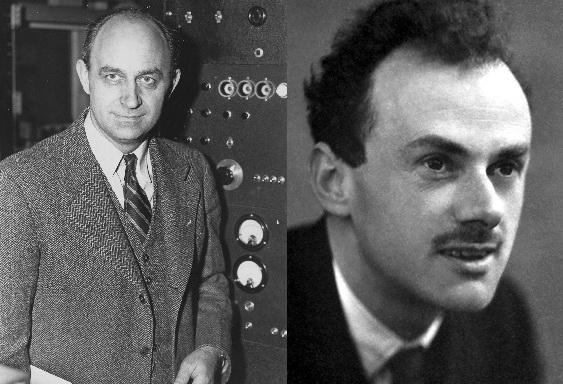
\includegraphics[width=0.4\textwidth]{./figures/Fermi-Dirac.jpg}};
        \node[inner sep=0pt] (Fermi) at (-2.35,-2.0) {\small Enrico Fermi};
        \node[inner sep=0pt] (Dirac) at (0.35,-2.0) {\small Paul Dirac};
      \end{tikzpicture}

      \vspace{1.0pt}

      \centering
      \begin{tikzpicture}
        \node[inner sep=0pt] (figure) at (0,0)
        {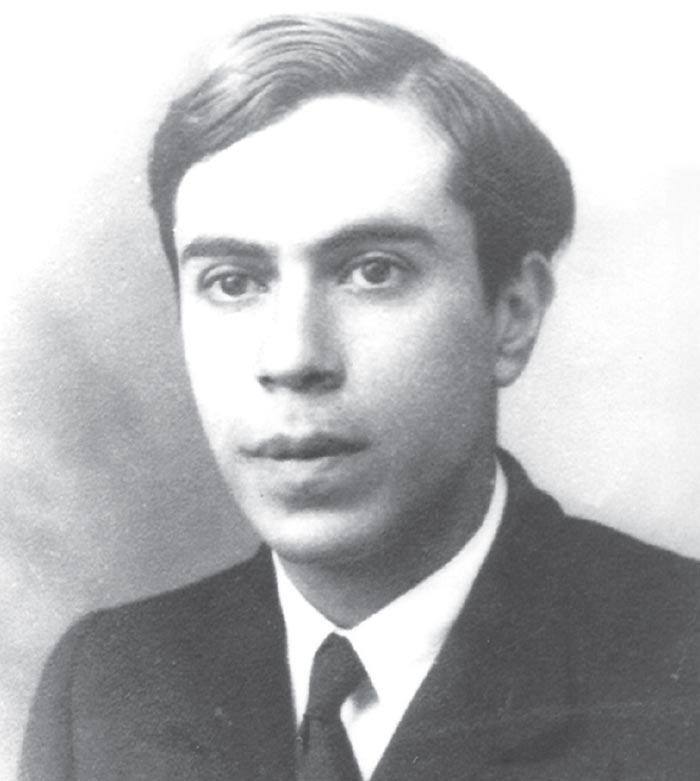
\includegraphics[width=0.18\textwidth]{./figures/Ettore_Majorana.jpg}};
        \node[inner sep=0pt] (Enrico) at (0,-1.65) {\small Ettore Majorana}
      \end{tikzpicture}

      \begin{itemize}
        \setlength\itemsep{0pt}
        \small
        \item Fermions
          \begin{itemize}
            \item Dirac, Weyl, Majorana
            \item Fermi-Dirac statistics
            \item Half-odd-integer spin
          \end{itemize}
      \end{itemize}
      \begin{itemize}
        \setlength\itemsep{0pt}
        \small
        \item  Dirac Fermions
        \begin{itemize}
          \item Particle $\neq$ Antiparticle
          \item Charged, Massive
        \end{itemize}
      \end{itemize}

      \begin{itemize}
        \setlength\itemsep{0pt}
        \small
        \item  Weyl Fermions
        \begin{itemize}
          \item Particle $\neq$ Antiparticle
          \item Charged, Massless
        \end{itemize}
      \end{itemize}

      \begin{itemize}
        \setlength\itemsep{0pt}
        \small
        \item Majorana Fermions (MFs)
        \begin{itemize}
            \item Particle $=$ Antiparticle
            \item Neutral, Massive
            \item SM candidates: Neutrino, Dark Matter
        \end{itemize}
      \end{itemize}

    \end{multicols}

  \end{frame}

  \begin{frame}{MFs in Particle Physics}
    \begin{multicols}{2}
      \centering
      \begin{tikzpicture}
        \node[inner sep=0pt] (figure) at (0,0)
        {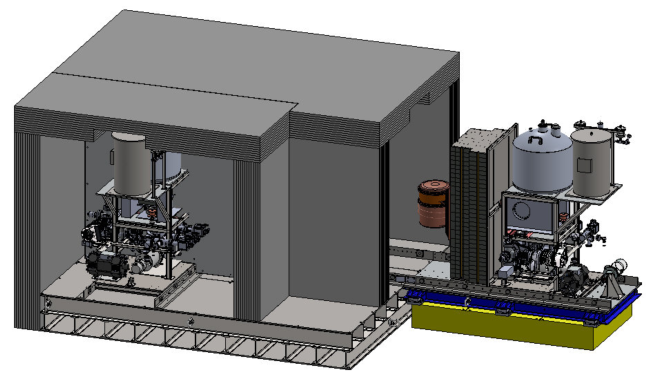
\includegraphics[width=0.5\textwidth]{./figures/majorana-experiment.png}};
        \node[inner sep=0pt] (reference) at (0,-2.1) {\small MAJORANA project:};
        \node[inner sep=0pt] (reference) at (0,-2.5) {\small neutrinoless double beta (0$\nu\beta\beta$) decay};
      \end{tikzpicture}

      \begin{itemize}
          \item Are neutrinos MFs?
          \item If yes, standard model is incomplete
          \item Negative results for Majorana particles so far
      \end{itemize}

    \end{multicols}
  \end{frame}

  \begin{frame}{MFs in Condensed Matter}
    \begin{multicols}{2}
      \begin{itemize}
        \item Superconductors (SCs)
          \begin{itemize}
            \item Cooper pairs
            \begin{itemize}
              \item Electron-phonon interaction pairs two electrons with opposite spin and momenta.
            \end{itemize}
            \pause
            \item Bogoliubov quasiparticles
            \begin{itemize}
              \item Excitation from ground state, pairs an electron to a hole with opposite momenta.
              \item[] \[ H_{BdG} = \begin{bmatrix} \epsilon(k) & \de(k) \\ \de^\ast(k) & -\epsilon(-k) \end{bmatrix} \]
              \item Zero-energy excitations in \textit{p}-wave SC may be MFs.
              \item Come in pairs.
            \end{itemize}
          \end{itemize}
      \end{itemize}
      \vspace{30mm}

      \begin{figure}
        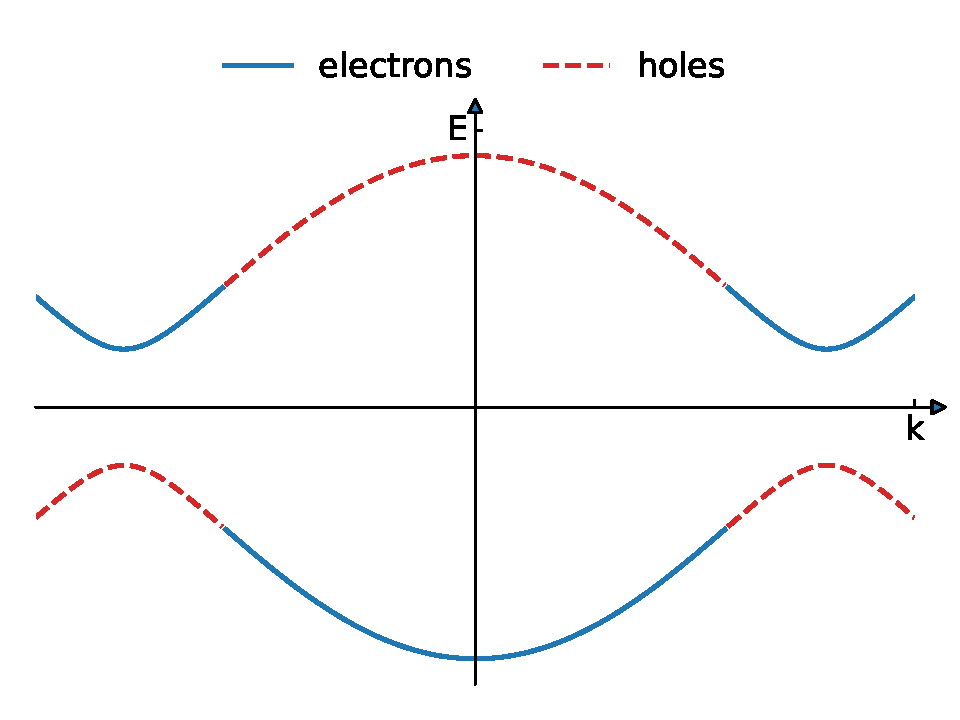
\includegraphics[width=0.50\textwidth]{./figures/p-wave-mu-p1_25.pdf}
      \end{figure}

    \end{multicols}

  \end{frame}

  %\begin{frame}
  %\frametitle{Topology in Condensed Matter}

  %\begin{multicols}{2}
  %\centering Topology
  %\begin{figure}
  %  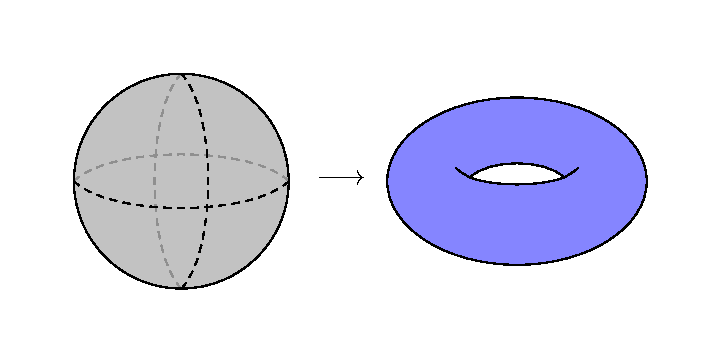
\includegraphics[width=0.5\textwidth]{./figures/topology.pdf}
  %\end{figure}
  %\pause
  %\vspace{10em}

  %\centering Topological States
  %\begin{figure}
  %  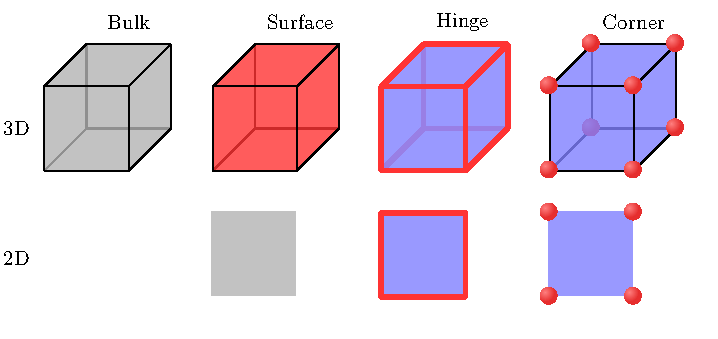
\includegraphics[width=0.5\textwidth]{./figures/topological-states.pdf}
  %\end{figure}

  %\end{multicols}
  %\end{frame}

  \begin{frame}{MFs in Condensed Matter}
    \begin{tikzpicture}
      \only<1>{\node[inner sep=0pt] (f1) at (0,0) {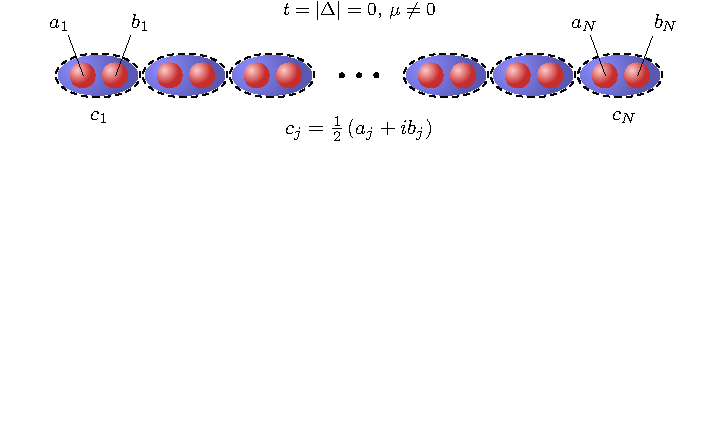
\includegraphics[width=0.9\textwidth]{./figures/kitaev-chain-1.pdf}};}
      \only<2>{\node[inner sep=0pt] (f2) at (0,0) {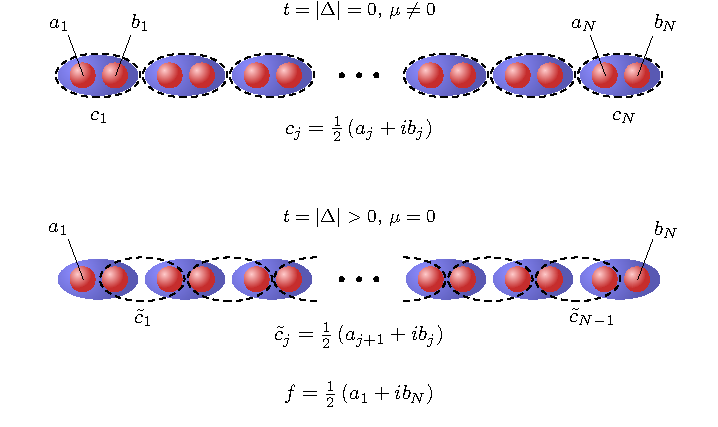
\includegraphics[width=0.9\textwidth]{./figures/kitaev-chain-2.pdf}};}
    \end{tikzpicture}
  \end{frame}

  %\begin{frame}{MFs in Condensed Matter}
  %  \begin{figure}
  %    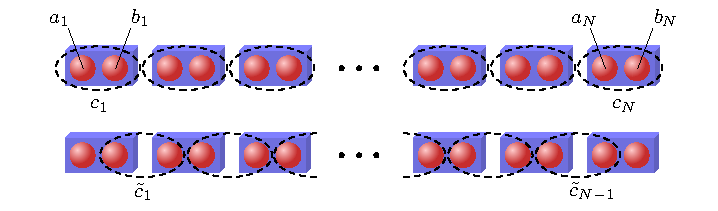
\includegraphics[width=\textwidth]{./figures/kitaev-chain.pdf}
  %  \end{figure}

  %  \vspace{20pt}
  %  Complex fermion in Majorana fermion basis
  %  \begin{equation}
  %    c_j = \dfrac{1}{2}(a_j + i b_j).
  %  \end{equation}

  %\end{frame}

  %\begin{frame}{MFs in Condensed Matter}
  %  Hamiltonian for a 1D tight-binding chain with spinless \textit{p}-wave superconductivity
  %  \begin{equation}
  %    \ham_{chain} = -\mu\sum_j^N \cc_j c_j -\sum_j^{N-1} t \cc_j c_{j+1} + |\de| c_j c_{j+1} + h.c.
  %  \end{equation}
  %  Hamiltonian in Majorana fermion basis
  %  \begin{equation}
  %    \ham_{chain} = \dfrac{i}{2} \sum_j -\mu a_j b_j + (t+|\de|) b_j a_{j+1} + (-t+|\de|) a_j b_{j+1}.
  %  \end{equation}
  %  $t=|\de|=0$ and $\mu<0$, trivial phase
  %  \begin{equation}
  %    \ham = -\dfrac{i\mu}{2} \sum_j a_j b_j.
  %  \end{equation}
  %  $t=|\de|>0$ and $\mu=0$, non-trivial (topological) phase
  %  \begin{equation}
  %    \ham = it \sum_j b_j a_{j+1}.
  %  \end{equation}

  %\end{frame}

  %\begin{frame}{MFs in Condensed Matter}
  %  \begin{figure}
  %    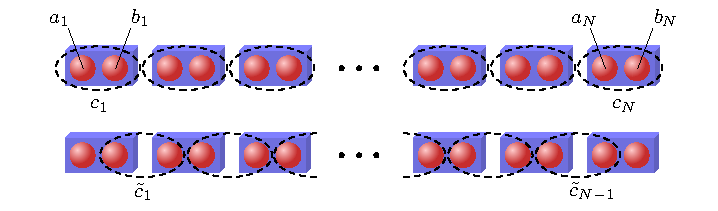
\includegraphics[width=\textwidth]{./figures/kitaev-chain.pdf}
  %  \end{figure}

  %  Intersite fermion representation
  %  \begin{equation}
  %    \tilde{c}_j = \dfrac{1}{2}(a_{j+1} + i b_j).
  %  \end{equation}
  %  The highly non-local fermion state
  %  \begin{equation}
  %    f = \dfrac{1}{2}(a_{1} + i b_N),
  %  \end{equation}
  %  corresponds to zero energy. This is still true for $|\mu|< 2t$.
  %\end{frame}

  \begin{frame}{Band Gaps and Topological Phase}
    \centering
    \begin{figure}
      \begin{tikzpicture}
        \node[inner sep=0pt] (tp) at (-4.6,0)
        {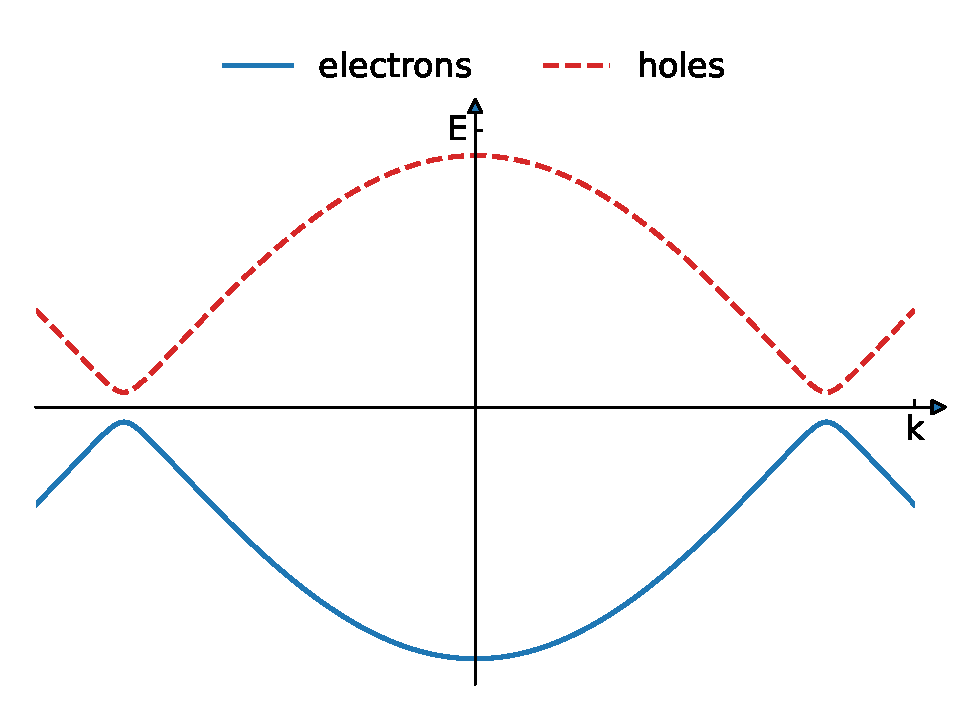
\includegraphics[width=0.33\textwidth]{./figures/p-wave-mu-p2_25.pdf}};
        \node[inner sep=0pt] (tp) at (-4.6,-2.0) {\footnotesize $\mu=2.25t$};
        \node[inner sep=0pt] (Mtp) at (-4.6,-2.5) {\footnotesize $\mathcal{M}=1$};
        \node[inner sep=0pt] (tp) at (-4.6,-3.0) {\footnotesize Trivial};

        \pause
        \node[inner sep=0pt] (cp) at (0,0)
        {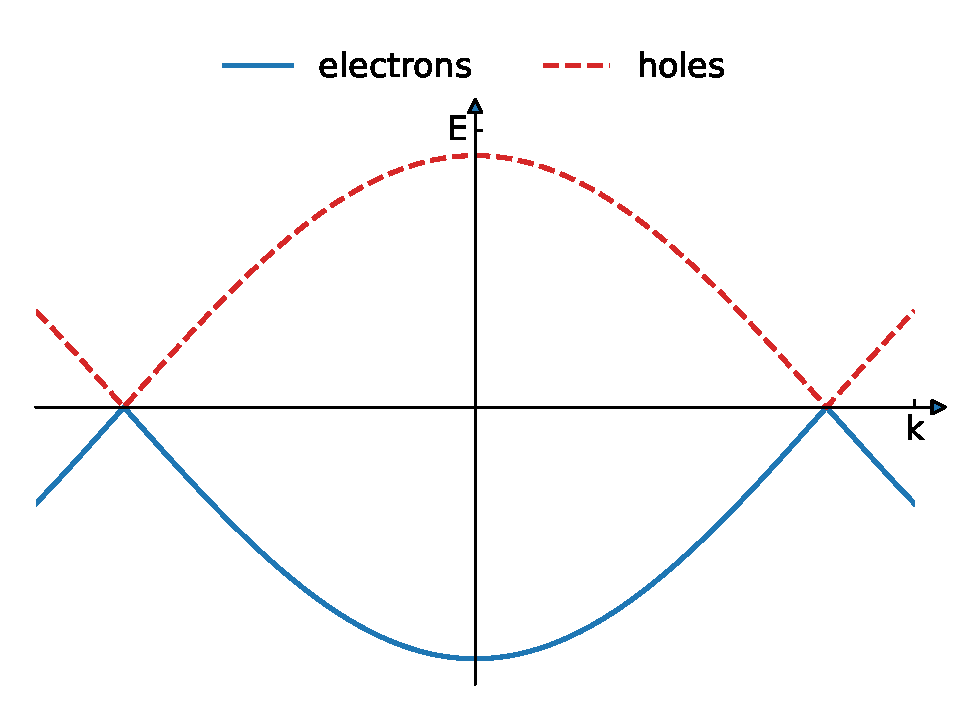
\includegraphics[width=0.33\textwidth]{./figures/p-wave-mu-p2_00.pdf}};
        \node[inner sep=0pt] (cp) at (0.0,-2.0) {\footnotesize $\mu_c=2t$};

        \pause
        \node[inner sep=0pt] (ntp) at (4.6,0)
        {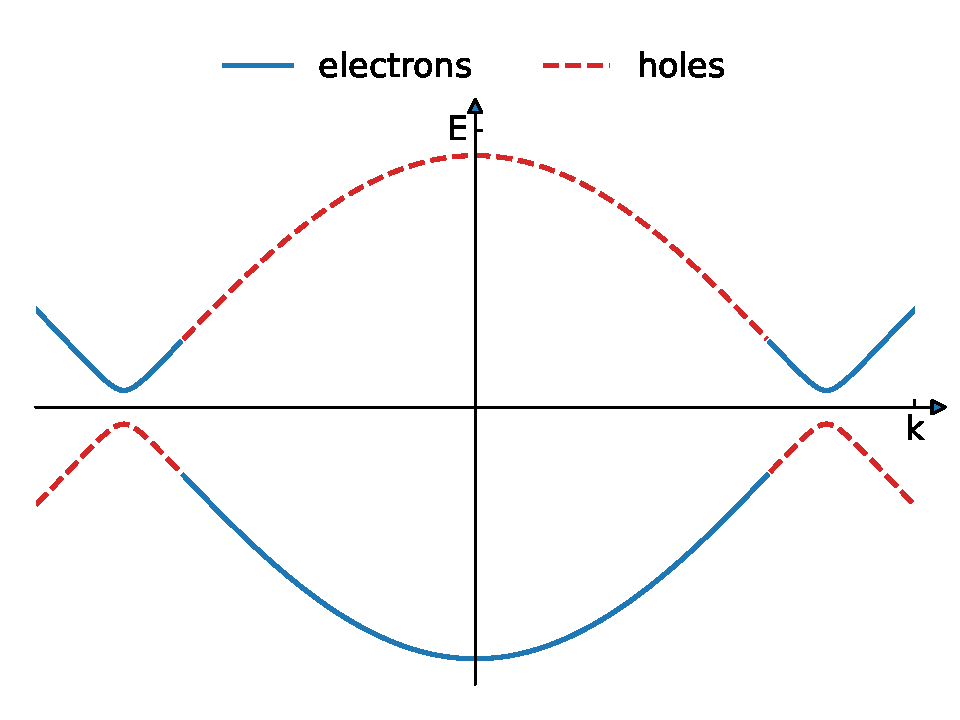
\includegraphics[width=0.33\textwidth]{./figures/p-wave-mu-p1_75.pdf}};
        \node[inner sep=0pt] (ntp) at (4.6,-2.0) {\footnotesize $\mu=1.75t$};
        \node[inner sep=0pt] (Mntp) at (4.6,-2.5) {\footnotesize $\mathcal{M}=-1$};
        \node[inner sep=0pt] (tp) at (4.6,-3.0) {\footnotesize Non-trivial};


      \end{tikzpicture}
    \end{figure}
    \visible<4>{
    \small
    \begin{itemize}
      \centering
      \item[] \underline{Non-trivial phase}
      \item[] \vspace{10pt}
      \begin{itemize}
        \centering
        \item[]Large band gap $\rightarrow$ Robust against local errors $\rightarrow$ Topologically protected
      \end{itemize}
    \end{itemize}}
  \end{frame}

  \begin{frame}{Majorana Number \& Bulk-Edge Correspondence}
    %Majorana number topological invariant 1D SC

    Transform to Majorana basis
    \begin{equation}
      A = -i U \ham U^{\dagger}
    \end{equation}
    Majorana number
    \begin{equation}
      \mathcal{M} = \text{sgn}[\text{Pf}(A)]
    \end{equation}

    %Particle-hole symmetry in momentum-space allows
    %\begin{equation}
    %  \mathcal{M} =
    %  \begin{cases}
    %    \text{sgn} [\text{Pf} (A_{k=0}) \text{Pf} (A_{k=\pi})], &\text{if L is even}      , \\
    %    \text{sgn} [\text{Pf} (A_{k=0})], &\text{if L is odd},
    %  \end{cases}
    %\end{equation}

    \begin{itemize}
      \item If $|\mu| > 2t$, $\mathcal{M} = +1$, trivial topology
      \item If $|\mu| < 2t$, $\mathcal{M} = -1$, non-trivial topology
    \end{itemize}
    \pause

    \begin{figure}
      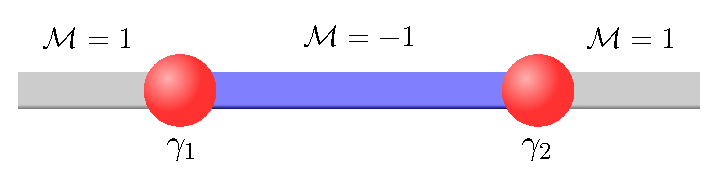
\includegraphics[width = 0.6\textwidth]{./figures/bulk-edge.pdf}
    \end{figure}


  \end{frame}

%  \begin{frame}{Effective \textit{p}-wave superconductor NEEDED?}
%    \begin{multicols}{2}
%      \centering
%      \begin{tikzpicture}
%        \node[inner sep=0pt] (figure) at (0,0)
%        {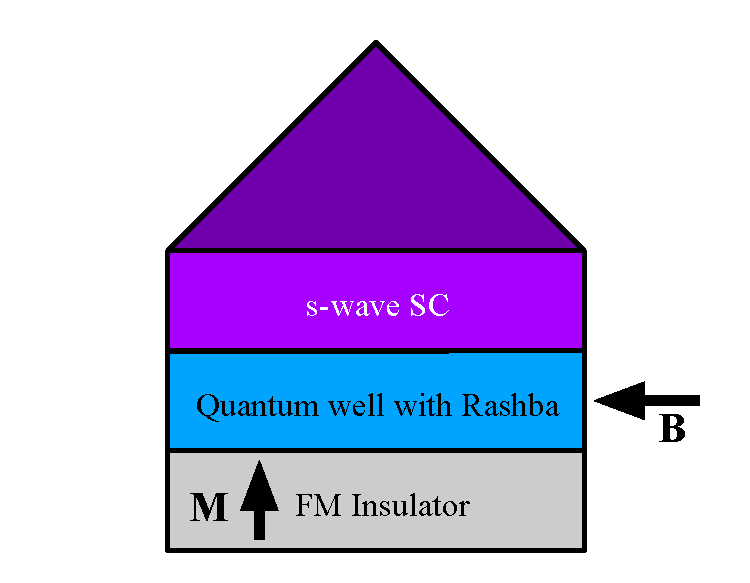
\includegraphics[width=0.5\textwidth]{./figures/tunable-semiconductor.pdf}};
%        \node[inner sep=0pt] (reference) at (0,-3) {\small Alicea, \textit{PRB} \textbf{81}, 125318 (2010).};
%      \end{tikzpicture}
%      \small
%      \begin{equation}
%        c_j = (c_{j\uparrow}, c_{j\downarrow})^T
%      \end{equation}
%      \textit{s}-wave SC paring term:
%      \begin{equation}
%        \ham_{SC} = \sum_j \de \cc_{j\uparrow} \cc_{j\downarrow} + h.c.
%      \end{equation}
%      Quantum well:
%      \begin{equation}
%        \ham_0 = \sum_j (6t - \mu) \cc_j c_j - \sum_{\langle j,l \rangle} (t \cc_l c_j + h.c.)
%      \end{equation}
%      Rashba spin-orbit coupling:
%      \begin{equation}
%        \ham_R = -it_R \sum_{\langle j,l \rangle \alpha\beta} \cc_{l\alpha} (\bm{\sigma}_{\alpha\beta} \times \hat{r}_{lj}) \cdot \hat{z} c_{j\beta}
%      \end{equation}
%      Zeeman field:
%      \begin{equation}
%        \ham_Z = \sum_j \cc_j \vec{V} \cdot \bm{\sigma} c_j
%      \end{equation}
%
%    \end{multicols}
%  \end{frame}

  \begin{frame}{MFs in Condensed Matter}
    \begin{multicols}{2}
      \centering
      \begin{tikzpicture}
        \node[inner sep=0pt] (figure) at (0,0)
        {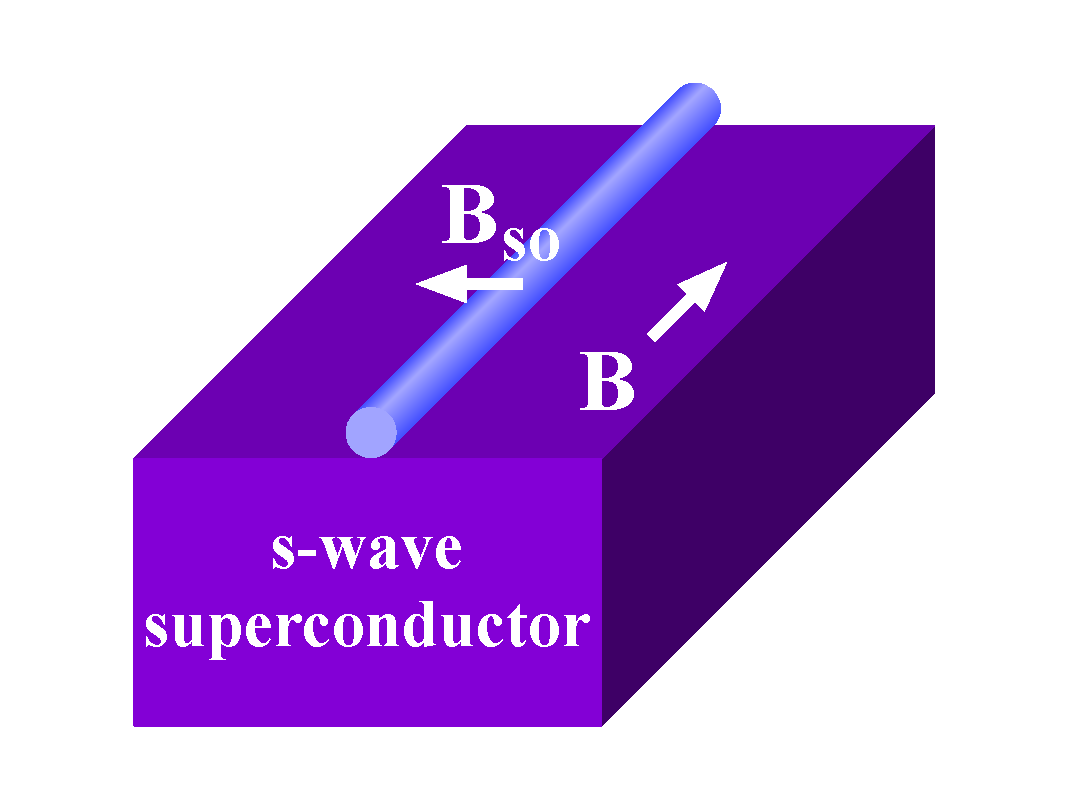
\includegraphics[width=0.35\textwidth]{./figures/swave-superconductor.pdf}};
      \end{tikzpicture}
      \begin{tikzpicture}
        \node[inner sep=0pt] (figure) at (0,0)
        {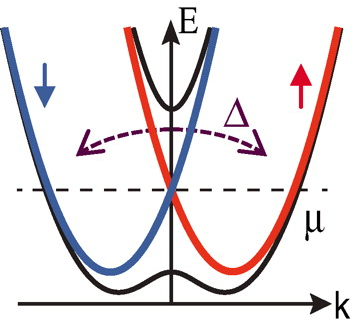
\includegraphics[width=0.30\textwidth]{./figures/Mourik-dispersion.jpeg}};
      \end{tikzpicture}
      \vspace{40pt}
      \begin{tikzpicture}
        \node[inner sep=0pt] (figure) at (0,0)
        {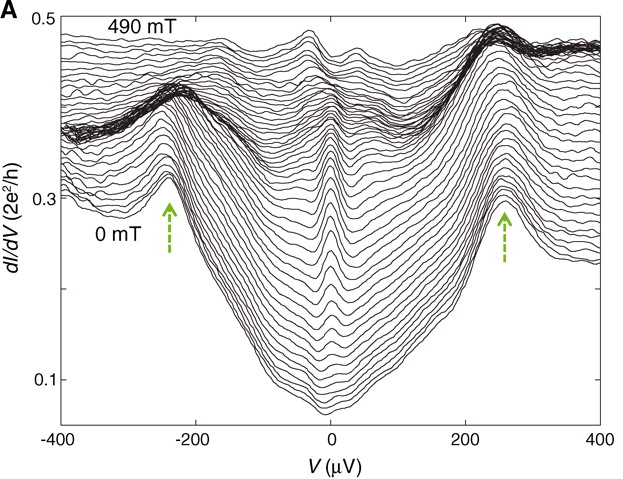
\includegraphics[width=0.50\textwidth]{./figures/Mourik-didv-curve.png}};
        \node[inner sep=0pt] (reference) at (0.25,-3) {\footnotesize Mourik et al., \textit{Science} \textbf{336}, 1003 (2012).};
      \end{tikzpicture}
    \end{multicols}
  \end{frame}

  \begin{frame}{MFs in Condensed Matter}
    \begin{tikzpicture}
      \node[inner sep=0pt] (figure) at (-4,0)
      {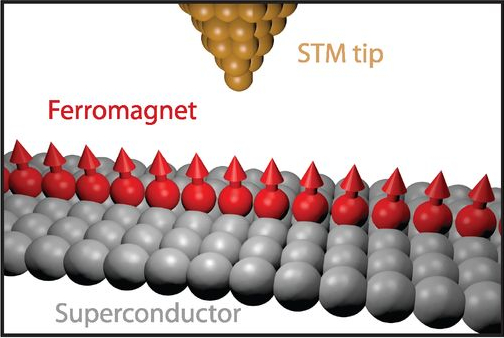
\includegraphics[width=0.5\textwidth]{./figures/Nadj-Perge-setup.png}};
      \node[inner sep=0pt] (figure) at (2.75,0)
      {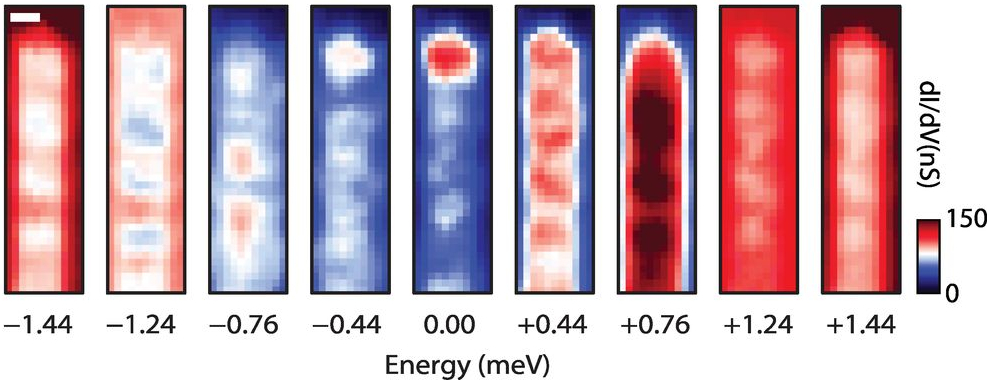
\includegraphics[width=0.5\textwidth]{./figures/Nadj-Perge-results.png}};
      \node[inner sep=0pt] (reference) at (2.75,-1.75) {\footnotesize Nadj-Perge et al., \textit{Science} \textbf{346}, 602 (2014).};
    \end{tikzpicture}
  \end{frame}

  \begin{frame}{MFs in Condensed Matter}
    \centering
    \begin{tikzpicture}
      \node[inner sep=0pt] (figure) at (0,0)
      {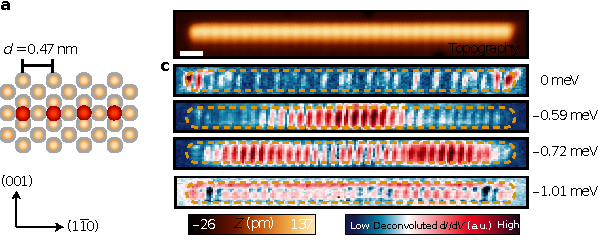
\includegraphics[width=\textwidth]{./figures/Schneider-results.pdf}};
      \node[inner sep=0pt] (reference) at (0,-3.00) {\footnotesize Mn atoms (red spheres) on top of superconducting Nb (brown spheres).};
      \node[inner sep=0pt] (reference) at (0,-3.40) {\footnotesize Schneider et al., \textit{Nature Nanotechnology} \textbf{17}, 384 (2022).};
    \end{tikzpicture}
  \end{frame}


  \section{\MO}

  %\begin{frame}{Braiding in a 2D \textit{p}-wave SC}
  %  \footnotesize
  %  \begin{multicols}{2}
  %    \begin{itemize}
  %      \item \textit{p}-wave superconductors can exhibit half-quantum vortices.
  %      \item Triplet pairing
  %        \begin{equation*}
  %          \vec{d}(\vec{k}) = \Delta e^{i\phi} \langle \cos \alpha, \sin \alpha, 0 \rangle(k_x + i k_y)
  %        \end{equation*}
  %      \item The order phase $\phi$ and angle $\alpha$ of $\vec{d}$ rotate by $\pi: (\phi,\vec{d}) \mapsto (\phi+\pi, -\vec{d})$.
  %      \item The order parameter $\theta$ maps to itself, $(0,2\pi)$, under the simultaneous change of both \vec{d} and $\phi: \theta = \phi+\alpha$.
  %    \end{itemize}
  %    \begin{equation*}
  %      \ham_{\Delta} = \int d^2\vec{r} \Delta \left[ \Psi^{\dagger} \left[ e^{i\theta} * (\partial_x + i\partial_y) \right] \Psi + h.c. \right]
  %    \end{equation*}
  %    %\vspace{20pt}

  %    \centering
  %    \begin{figure}
  %      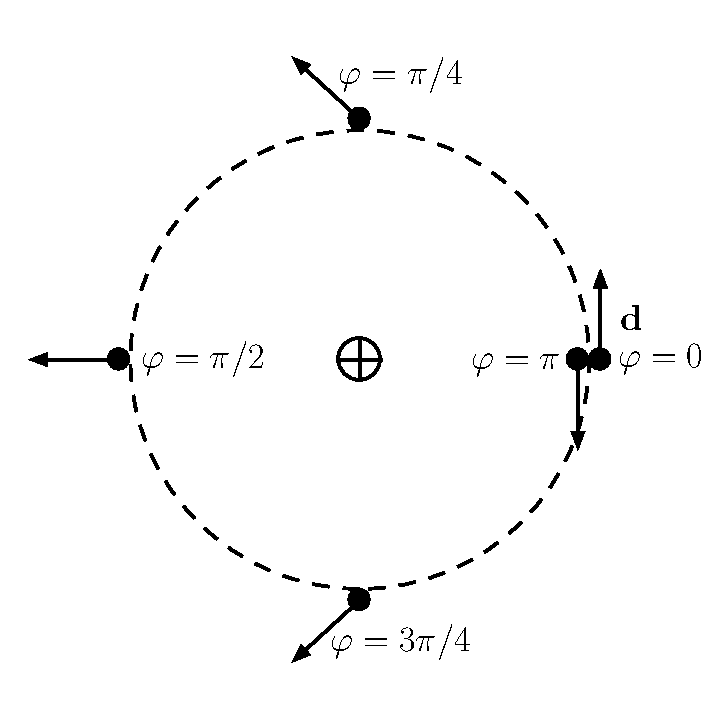
\includegraphics[width=0.45\textwidth]{./figures/half-quantum-vortex.pdf}
  %    \end{figure}

  %    \begin{itemize}
  %      \item if overall phase shifts by $\theta:$ $\Psi_{\alpha} \mapsto e^{i\theta/2} \Psi_{\alpha}$.
  %      \item $(u,v) \mapsto (u e^{i\theta/2}, v e^{-i\theta/2})$
  %    \end{itemize}

  %  \end{multicols}
  %\end{frame}


  %\begin{frame}{Braiding in a 2D \textit{p}-wave SC}
  %  \begin{multicols}{2}
  %    \begin{figure}
  %      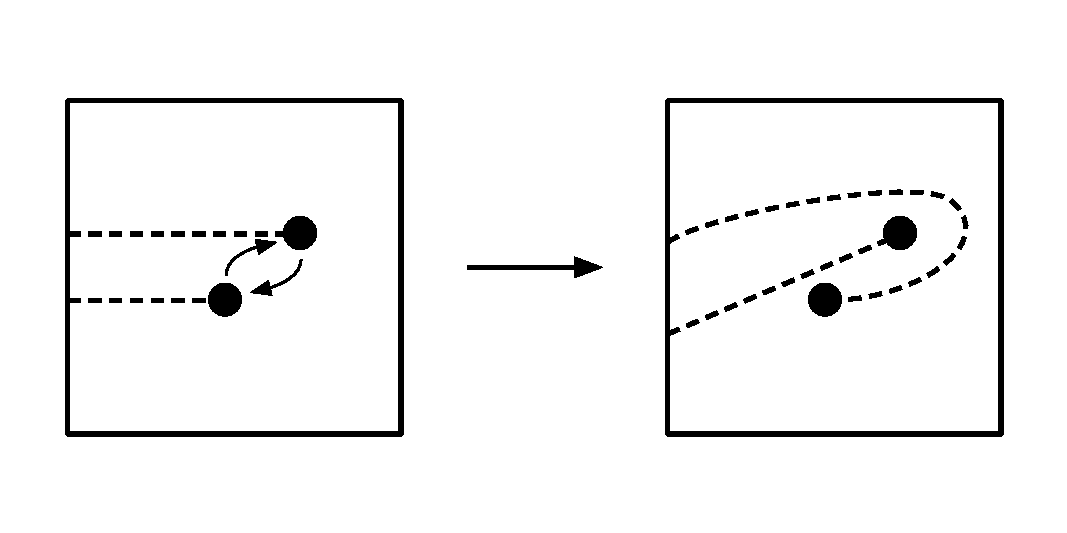
\includegraphics[width=0.5\textwidth]{./figures/pwave-braid.pdf}
  %    \end{figure}

  %    \begin{itemize}
  %        \item Interchanging two MFs:
  %        \begin{itemize}
  %          \item[] $\gamma_1 \rightarrow \gamma_2$ \\
  %          \item[] $\gamma_2 \rightarrow -\gamma_1$ \\
  %        \end{itemize}
  %        \item Exhibit Non-Abelian Statistics
  %        \item $a \ast b \neq b \ast a$
  %    \end{itemize}
  %    \begin{equation*}
  %    \end{equation*}
  %    \vspace{20pt}

  %    \centering
  %    \begin{tikzpicture}
  %      \node[inner sep=0pt] (figure) at (0,0)
  %      {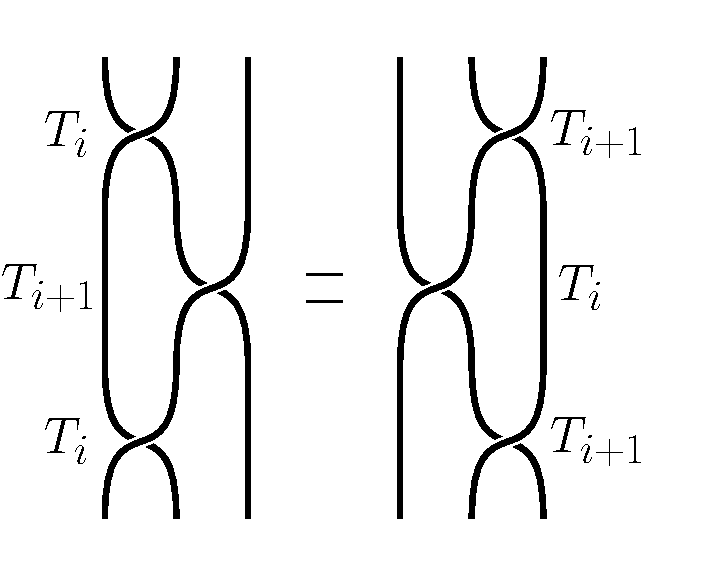
\includegraphics[width=0.45\textwidth]{./figures/braid.pdf}};
  %      \node[inner sep=0pt] (math) at (-0.18, -2.5) {\small $T_i T_j = T_j T_i$};
  %      \node[inner sep=0pt] (math) at (0, -3.0) {\small $T_i T_{i+1} T_i = T_{i+1} T_i T_{i+1}$};
  %      \node[inner sep=0pt] (reference) at (0,-3.5) {\footnotesize Ivanov, \textit{PRL} \textbf{86}, 268 (2001).};
  %    \end{tikzpicture}

  %  \end{multicols}
  %\end{frame}

  \begin{frame}{Braiding in 2D \textit{p}-wave SC}
    \small
    \begin{itemize}
      \item 2D \textit{p}-wave (triplet pairing) SC can exhibit half-quantum vortices.
        \vspace{1em}
      \pause
      \item Allows for MF states to accumulate $e^{i\theta/2}$ phase.
        \vspace{1em}
      \pause
      \item Braiding demonstrates non-Abelian statistics i.e.\ $A*B \neq B*A$,
        \begin{itemize}
          \item[\rightarrow] Allows for a universal quantum computer.
        \end{itemize}
        \vspace{1em}
      \pause
      \item Combine with MFs topological protection,
        \begin{itemize}
          \item[\rightarrow] Fewer qubits or operations required compared to modern qubits.
        \end{itemize}
    \end{itemize}
  \end{frame}

  \begin{frame}{Braiding in a Topological Quantum Computer}
      \begin{figure}
        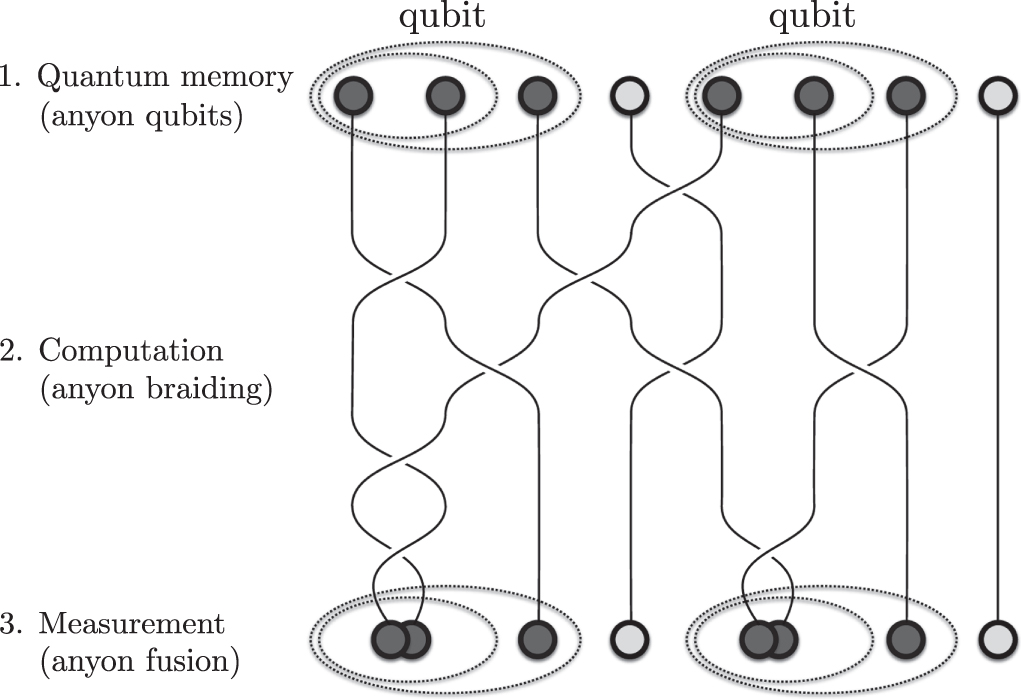
\includegraphics[width=0.65\textwidth]{./figures/braiding.jpg}
        \caption*{\footnotesize Field et.\ al., \textit{Quantum Sci. Technol.} \textbf{3}, 045004 (2018).}
      \end{figure}

  \end{frame}

  \begin{frame}{T-junction as a Quantum Logic Gate}

    \begin{multicols}{3}
    \begin{figure}
      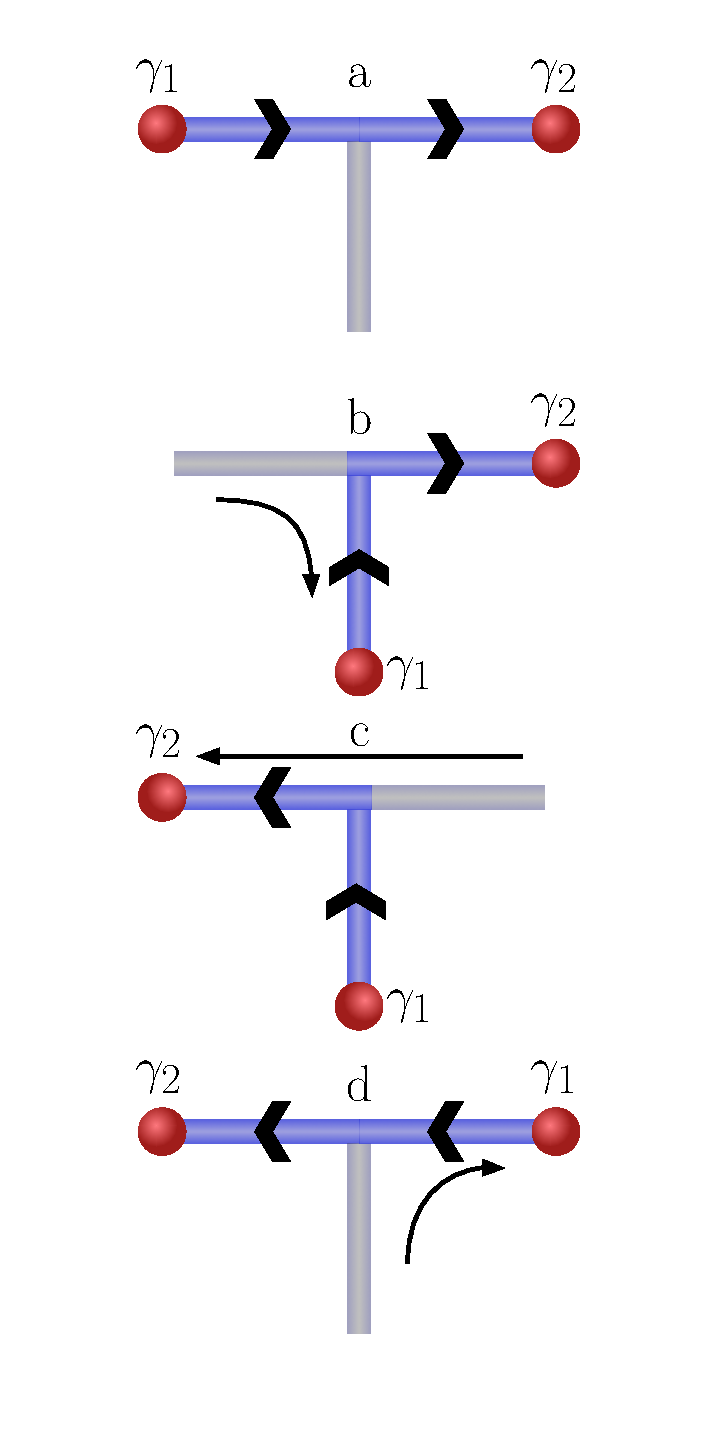
\includegraphics[width=0.30\textwidth]{./figures/t-junction-braid.pdf}
    \end{figure}

      \begin{minipage}{0.67\textwidth}
      \small
      %\begin{equation}
      %  \ham_T = -\mu \sum_j \cc_j c_j - \sum_j t \cc_j c_{j+1} + |\de| e^{i\phi} c_j c_{j+1} + h.c.
      %\end{equation}
      %\begin{equation}
      %  c_j = e^{-i(\phi/2)}(\gamma_{j+1,1} + i \gamma_{j,2})/2
      %\end{equation}
      \vspace{4em}
      \begin{itemize}
        \footnotesize
        \item Take pairing term $|\de|e^{i\phi} c_j c_{j+1}$ such that the site indices:
        \item Increase moving $\rightarrow / \uparrow$ in the horizontal/vertical wires: $\phi=0$,
        \item Decrease moving $\leftarrow / \downarrow$ in the horizontal/vertical wires: $\phi=\pi$.
      \end{itemize}

      \centering
      \begin{tikzpicture}
        \node[inner sep=0pt] (figure) at (0,0)
        {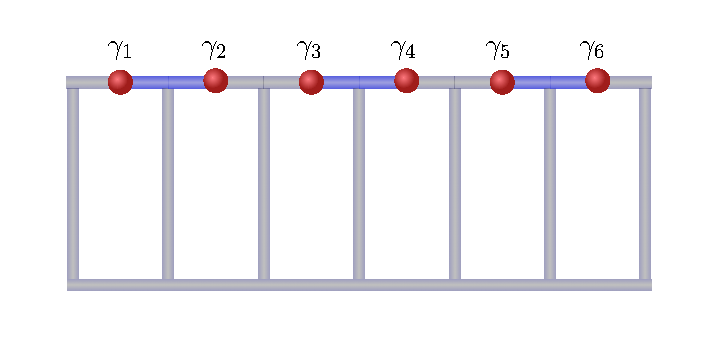
\includegraphics[width=0.8\textwidth]{./figures/ladder-junction.pdf}};
        \node[inner sep=0pt] (reference) at (0,-1.5) {\small Alicea et al., \textit{Nature Phys.} \textbf{7}, 412 (2011)}
      \end{tikzpicture}
      \vspace{20cm}
      \end{minipage}

    \end{multicols}
  \end{frame}

  \begin{frame}
    \frametitle{Triangular Structures for Braiding}
    \begin{multicols}{2}

    \begin{itemize}
      \item Consider triangular islands, topologically similar to T-junctions.
      \item Islands of three-fold rotational symmetry occur naturally in epitaxial growth on close-packed metal surfaces.
      \item Make a smooth connection from 1D to 2D superconductors.
    \end{itemize}
    \newline

    \begin{figure}
      \begin{tikzpicture}
        \node[inner sep=0pt] (figure) at (0,0)
        {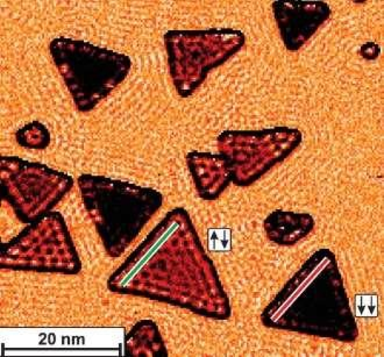
\includegraphics[width=0.4\textwidth]{./figures/triangular-islands.pdf}};
        \node[inner sep=0pt] (caption) at (0,-2.8) {\scriptsize Triangular Co islands on Cu(111).};
        \node[inner sep=0pt] (reference) at (0,-3.2) {\small Pietzsch et al., \textit{PRL} \textbf{96}, 237203 (2006)}
        \end{tikzpicture}
      \end{figure}
    \end{multicols}

  \end{frame}

  \begin{frame}{Topological phase transition induced by a supercurrent}
    \centering
    \begin{tikzpicture}
      \node[inner sep=0pt] (figure) at (0.0,1.5)
      {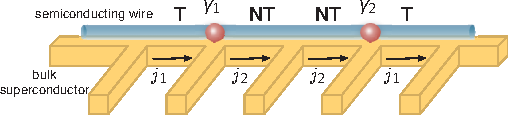
\includegraphics[width=0.6\textwidth]{./figures/Romito-setup.pdf}};
      \node[inner sep=0pt] (figure2) at (0.0,-2.0)
      {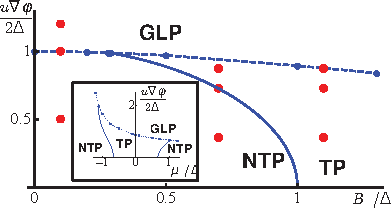
\includegraphics[width=0.6\textwidth]{./figures/Romito-topology-map2.pdf}};
      \node[inner sep=0pt] (reference) at (0,-4.5) {\small Romito et al., \textit{PRB} \textbf{85}, 020502(R) (2012).};
    \end{tikzpicture}
  \end{frame}

  \begin{frame}{Topological phase transition induced by a supercurrent}
    \centering
    \begin{tikzpicture}
      \node[inner sep=0pt] (figure) at (-3.5,0)
      {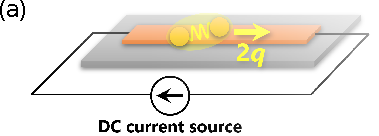
\includegraphics[width=0.4\textwidth]{./figures/Takasan-setup.pdf}};
      \node[inner sep=0pt] (figure2) at (3.0,0.0)
      {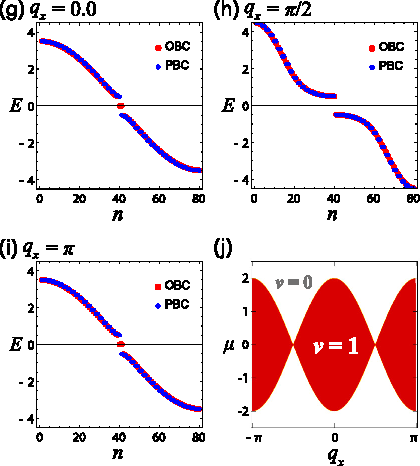
\includegraphics[width=0.5\textwidth]{./figures/Takasan-results.pdf}};
      \node[inner sep=0pt] (reference) at (-3.5,-1.5) {\small Takasan et al., \textit{PRB} \textbf{106}, 014508 (2022).};
    \end{tikzpicture}
  \end{frame}

  \section{\RE}

  \begin{frame}{Two Proposals}
    \begin{itemize}
      \item Exactly solvable ``Kitaev Triangle''
        \begin{itemize}
          \item[]
          \item Three fermion sites
          \item[]
          \item Three edges controlled by Peierls phase
        \end{itemize}
      \item[]
      \pause
      \item Finite-size triangle with hollow interior
        \begin{itemize}
          \item[]
          \item Under uniform vector potential
          \item[]
          \item Bulk-edge correspondence
        \end{itemize}
    \end{itemize}
  \end{frame}

  \begin{frame}{Kitaev Triangle}
    \footnotesize
    \begin{multicols}{2}
      \begin{figure}
        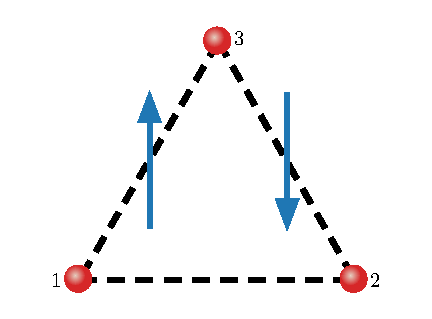
\includegraphics[width=0.4\textwidth]{./figures/3-point-triangle.pdf}
      \end{figure}
      \begin{equation}
        \vec{A} = \left[1-2\Theta(x) \right] \dfrac{2\pi}{3\sqrt{3}} \hat{y}
      \end{equation}
      \pause
      \begin{align}
        \cc_j c_l &\rightarrow \cc_j c_l \exp \left(\dfrac{i e}{\hbar} \int_{r_j}^{r_l} \vec{A} \cdot d\vec{l} \right) \nonumber \\
        &\rightarrow \cc_j c_l e^{i \phi_{jl}}
      \end{align}
      \begin{equation} \label{eq: Peierls chain}
        \ham = \sum_{\langle j,l\rangle} (-t e^{i\phi_{jl}} \cc_j c_l + \de \cc_j\cc_l + h.c.) - \mu \cc_j c_j
      \end{equation}
    \end{multicols}

    \pause
    In Kitaev limit, $t=\de\neq0$ and $\mu=0$,
    \begin{equation}
      (\phi_{12}, \phi_{23}, \phi_{31}) = (0, -\tfrac{\pi}{3}, -\tfrac{\pi}{3}) = \bm\phi_1
    \end{equation}
    MZMs localized at sites 1 and 2

  \end{frame}

  \begin{frame}{Kitaev Triangle Braiding}
    \footnotesize
    A closed parameter path linearly interpolated between the following sets of $\phi_{jk}$:
    \begin{equation}
      (\phi_{12}, \phi_{23}, \phi_{31}) : \bm\phi_1 \rightarrow \bm\phi_2 \rightarrow \bm\phi_3 \rightarrow \bm\phi_1
    \end{equation}

    \begin{tikzpicture}
      \node[inner sep=0pt] (figure) at (-3.5,0.35)
      {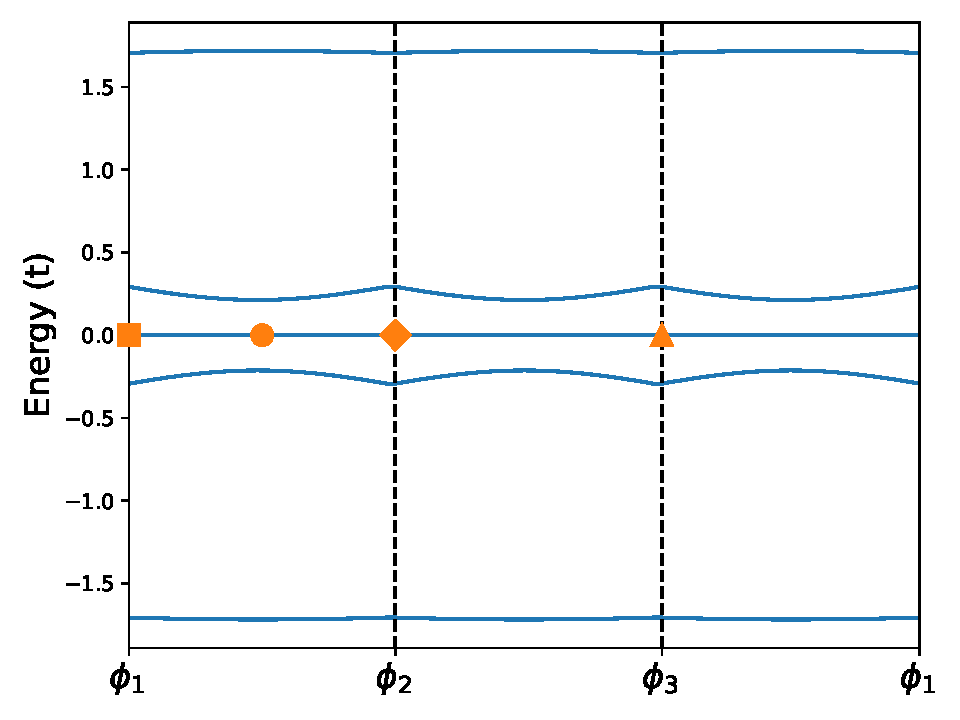
\includegraphics[width=0.5\textwidth]{./figures/3eigval.pdf}};
      \node[inner sep=0pt] (figure) at (3.6,0)
      {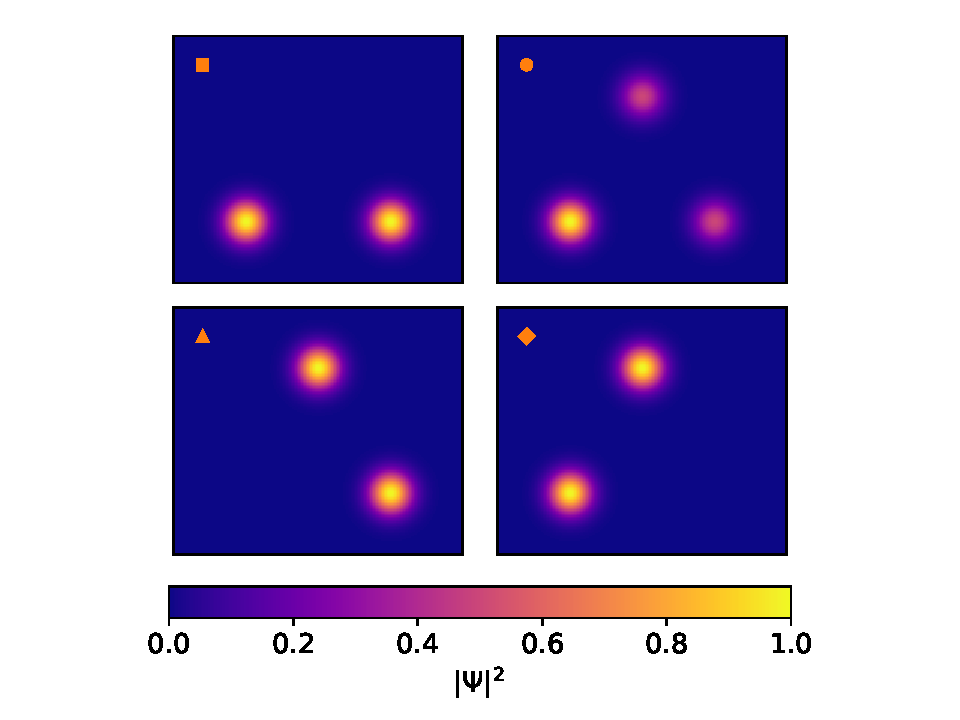
\includegraphics[width=0.6\textwidth]{./figures/3eigvec.pdf}};
    \end{tikzpicture}

  \end{frame}

  \begin{frame}
    \frametitle{Triangular Ribbon and Topological Phases}
    % show spectral plot and wavefunction

    \begin{multicols}{2}
      \small
      \begin{equation*}
        \phi_{jl} = \dfrac{e}{\hbar}\int_{\vec{r}_j}^{\vec{r}_l} \vec{A} \cdot d\vec{l} = \vec{A}\cdot\vec{r}_{jl} = -\phi_{lj}
      \end{equation*}
      \vspace{-08mm}
      \begin{figure}
        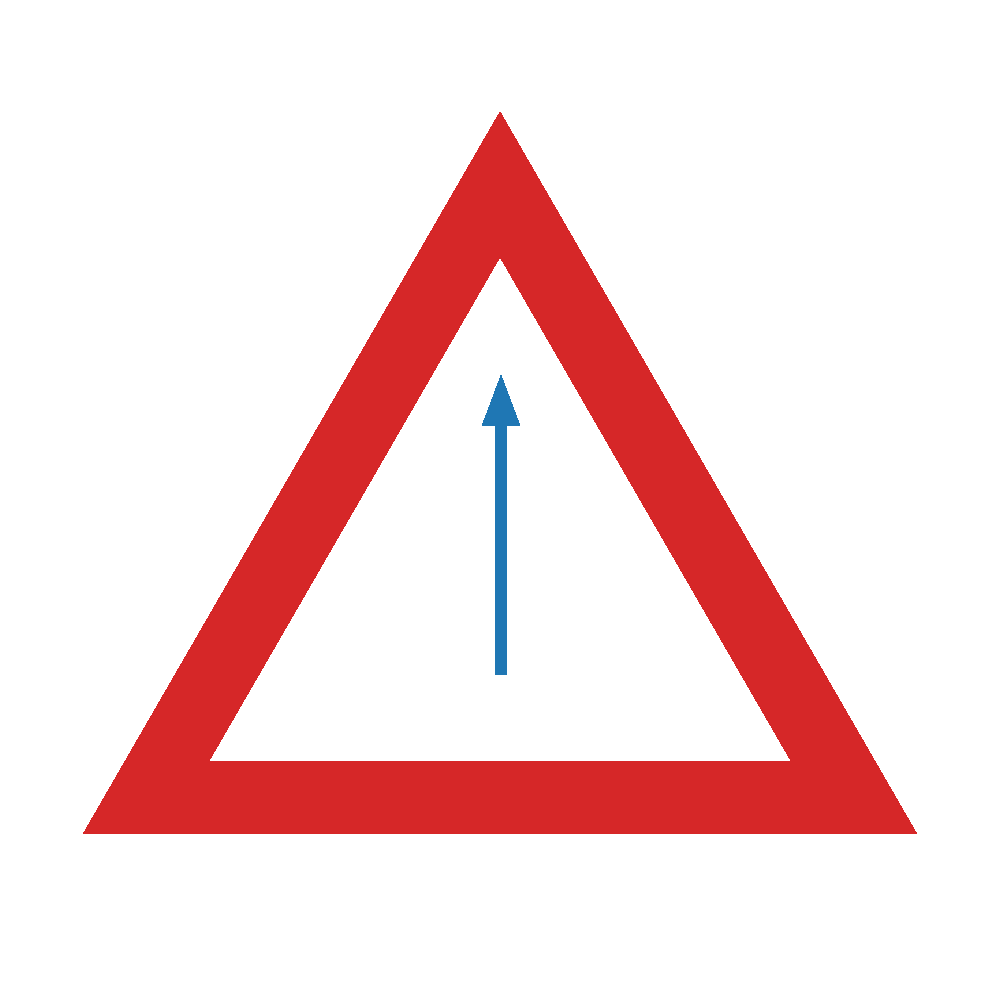
\includegraphics[width=0.30\textwidth]{./figures/hollow-triangle-constant-vector-potential.pdf}
      \end{figure}

      \vspace{-15mm}
      \begin{figure}
        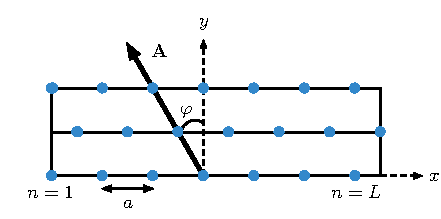
\includegraphics[width=0.3\textwidth]{./figures/triangular-lattice-finite-width-ribbon.pdf}
      \end{figure}

      \pause

      \begin{figure}
        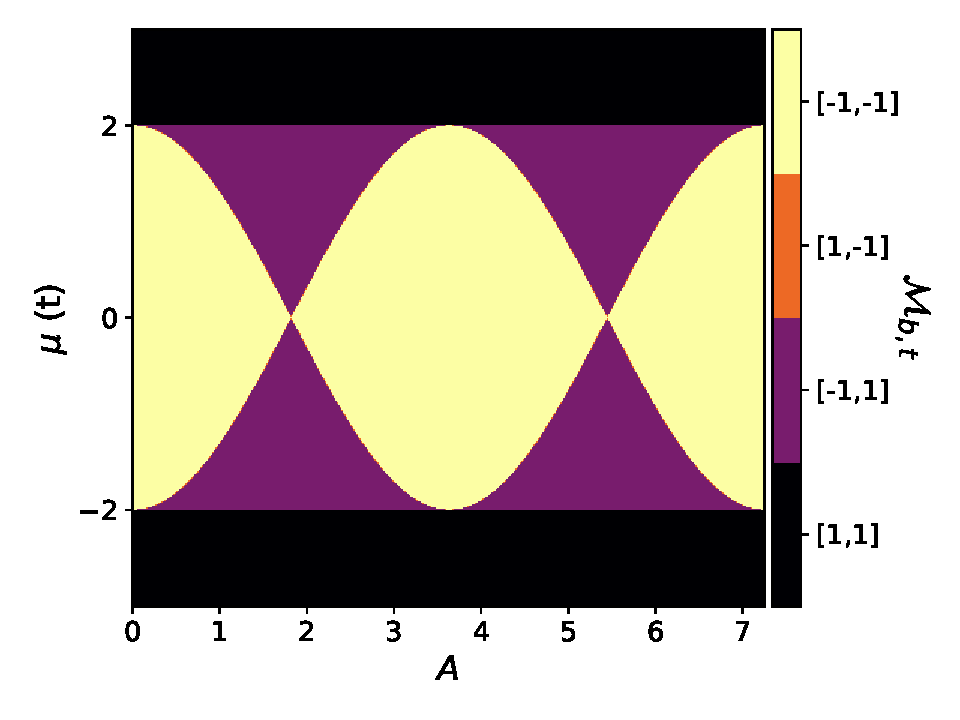
\includegraphics[width=0.4\textwidth]{./figures/topological-phase-diagram-1pi3-w-1.pdf} \\
        \hspace{-10mm}
        \pause
        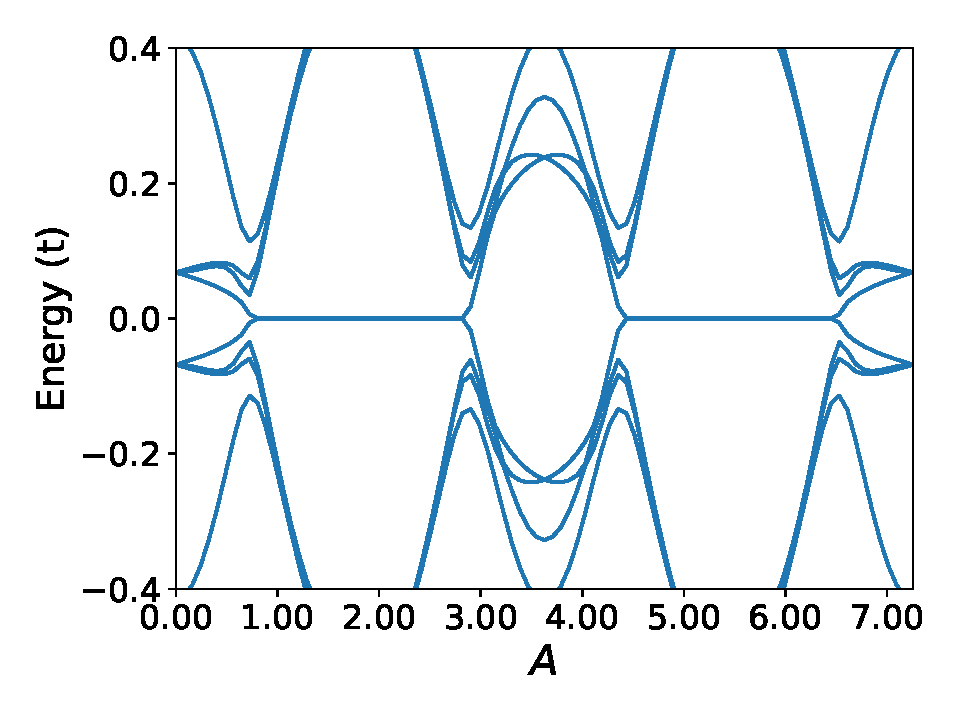
\includegraphics[width=0.34\textwidth]{./figures/spectral-flow-nr-50-w-1-mu-1_6.pdf}
      \end{figure}
    \end{multicols}

  \end{frame}

  \begin{frame}
    \frametitle{Rotating MFs on a Triangular Chain (W=1)}

    \begin{figure}
      \begin{tikzpicture}
        \node[inner sep=0pt] (figure) at (-2.8,0){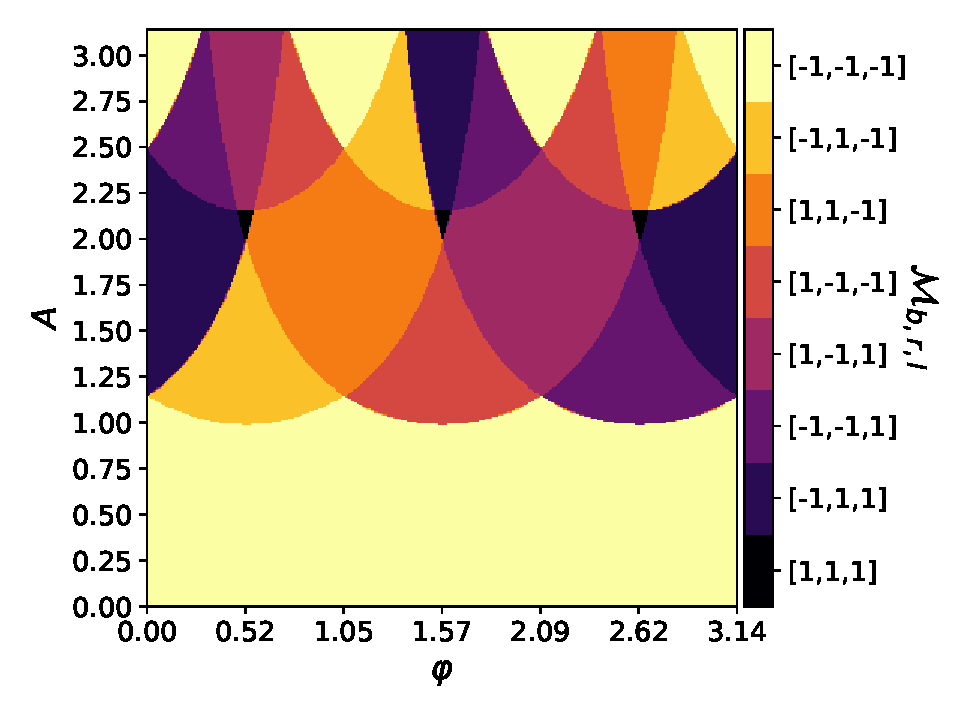
\includegraphics[width=0.4\textwidth]{./figures/topological-phase-diagram-w-1-mu-p1_1000.pdf}};
        \pause
        \draw[line width=0.3mm, green] (-4.62,1) -- (-1.4,1);
        \pause
        \node[inner sep=0pt] (figure2) at (2.8,0){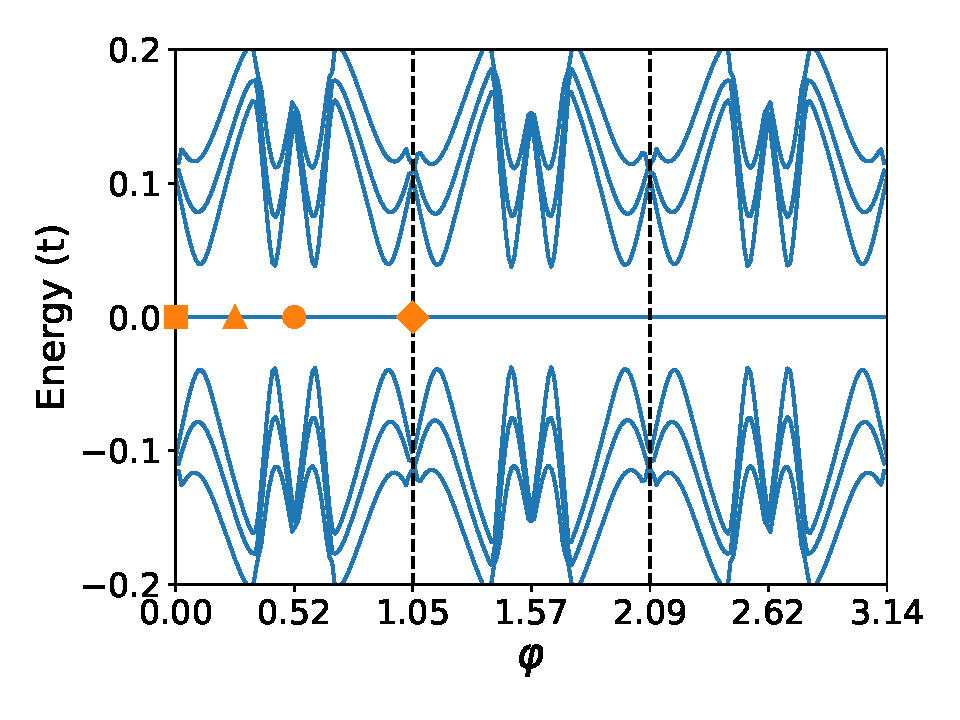
\includegraphics[width=0.4\textwidth]{./figures/spectral-flow-rotation-constant-vector-nr-50-w-1-mu-1_1.pdf}};
        \node[inner sep=0pt] (caption) at (0,-2.0) {\footnotesize $L=50$, $W=1$, $\mu=1.1$, $A=2.35$};
        \onslide<1->
      \end{tikzpicture}
    \end{figure}
    \pause
    \begin{figure}
      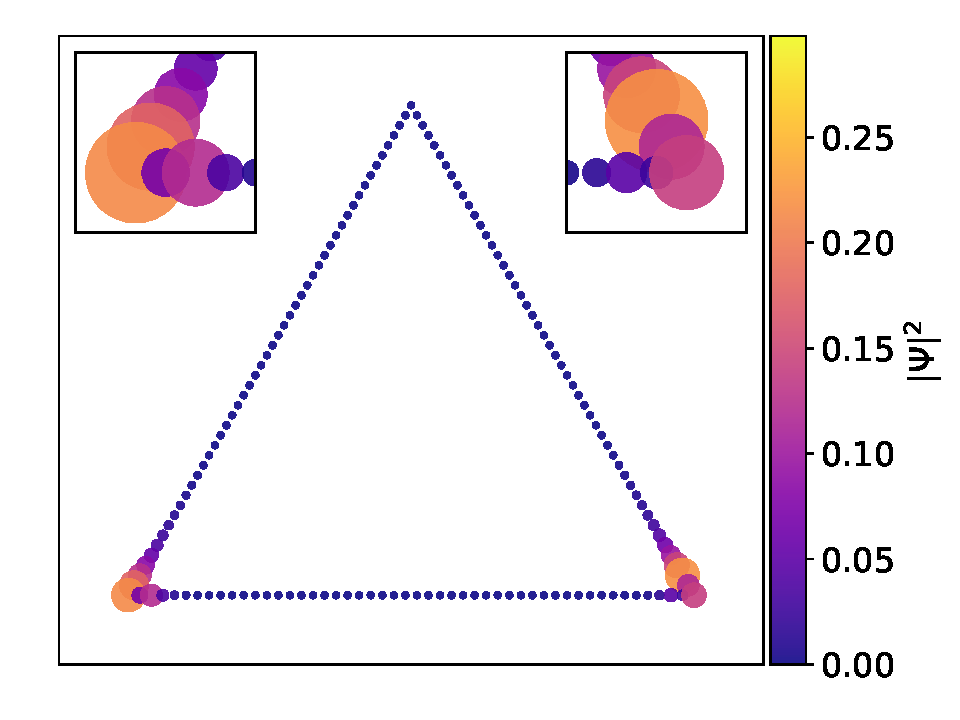
\includegraphics[height=80pt]{./figures/GS-T-Square.pdf}\hspace{-25pt}
      \pause
      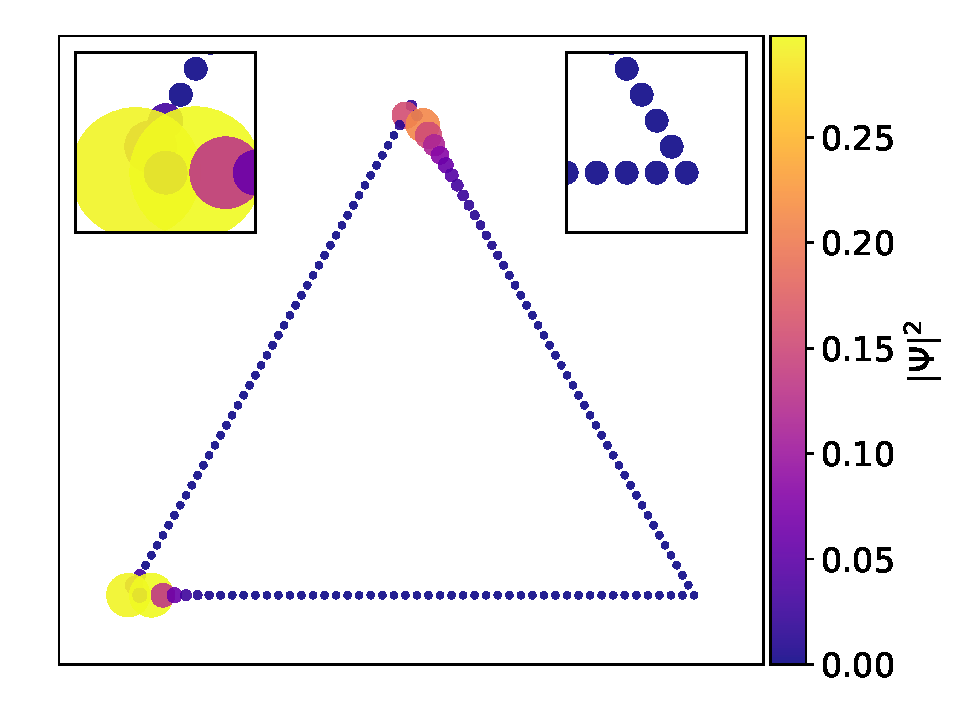
\includegraphics[height=80pt]{./figures/GS-T-Triangle.pdf}\hspace{-25pt}
      \pause
      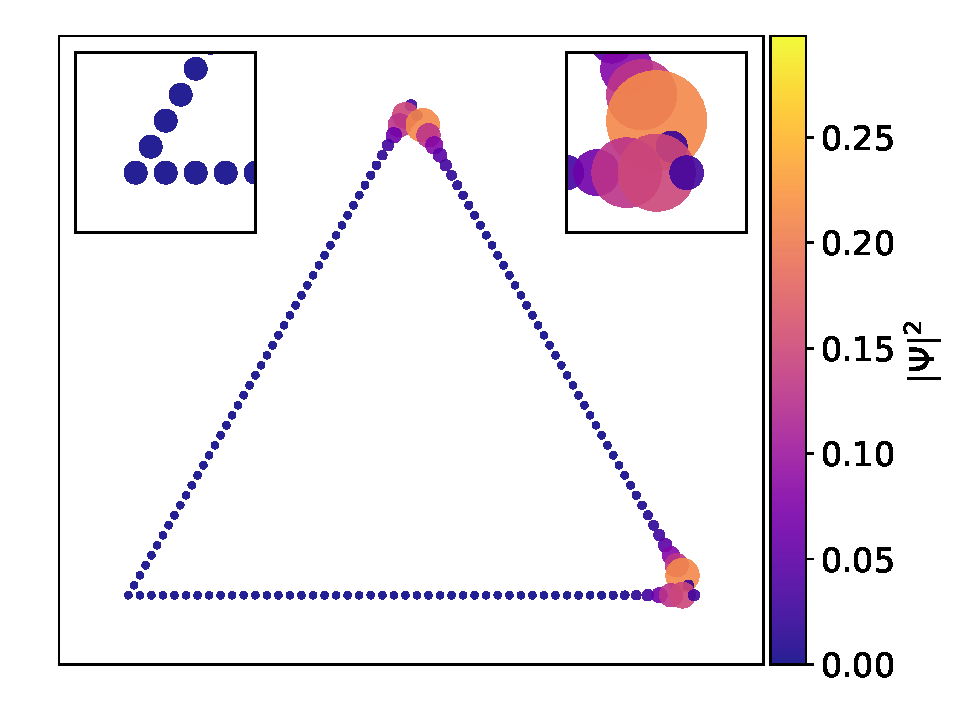
\includegraphics[height=80pt]{./figures/GS-T-Circle.pdf}\hspace{-25pt}
      \pause
      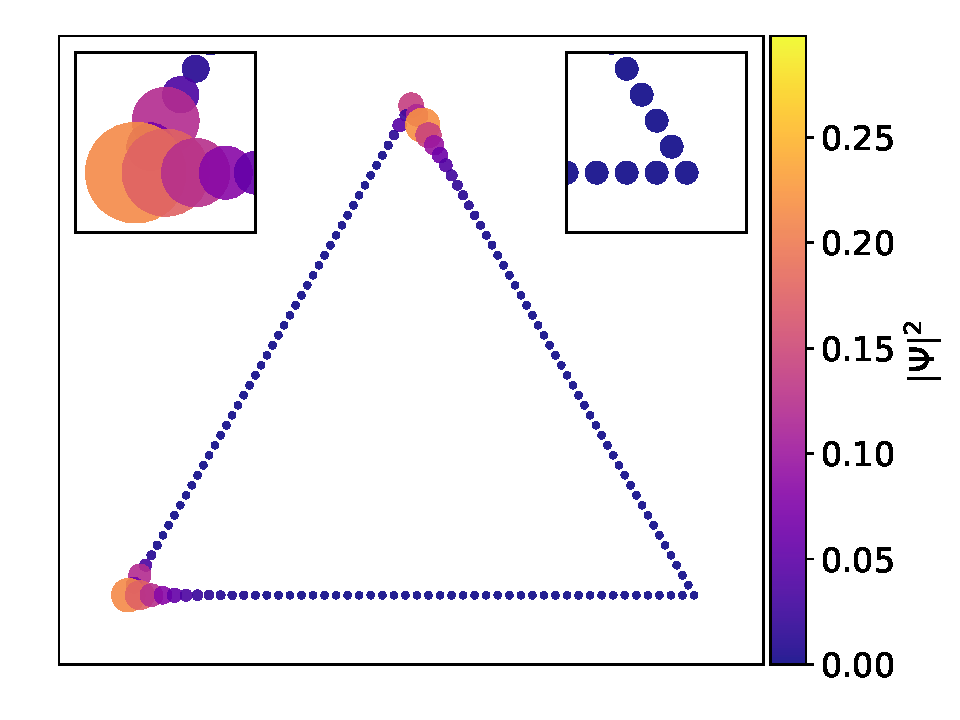
\includegraphics[height=80pt]{./figures/GS-T-Diamond.pdf}
    \end{figure}
  \end{frame}

  \begin{frame}
    \frametitle{Rotating MFs on a Hollow Triangle (W=3)}

    \begin{figure}
      \begin{tikzpicture}
        \node[inner sep=0pt] (figure) at (-4.4,0.0){\includegraphics[width=0.33\textwidth]{./figures/topological-phase-diagram-w-3-mu-p1_6000.pdf}};
        \node[inner sep=0pt] (figure2) at (0,0){\includegraphics[width=0.33\textwidth]{./figures/band-gap-rotation-w-3-mu-p1_6000.pdf}};
        \pause
        \draw[line width = 0.2mm, green] (-5.9,-0.43) -- (-5.45,-0.51);
        \draw[line width = 0.2mm, green] (-5.45,-0.51) -- (-5.01,-0.43);
        \draw[line width = 0.2mm, green] (-5.01,-0.43) -- (-4.56,-0.51);
        \draw[line width = 0.2mm, green] (-4.56,-0.51) -- (-4.13,-0.43);
        \draw[line width = 0.2mm, green] (-4.13,-0.43) -- (-3.68,-0.51);
        \draw[line width = 0.2mm, green] (-3.68,-0.51) -- (-3.25,-0.43);
        \draw[line width = 0.2mm, green] (-1.50,-0.43) -- (-1.05,-0.51);
        \draw[line width = 0.2mm, green] (-1.05,-0.51) -- (-0.56,-0.43);
        \draw[line width = 0.2mm, green] (-0.56,-0.43) -- (-0.07,-0.51);
        \draw[line width = 0.2mm, green] (-0.07,-0.51) -- (0.39,-0.43);
        \draw[line width = 0.2mm, green] (0.39,-0.43) -- (0.86,-0.51);
        \draw[line width = 0.2mm, green] (0.86,-0.51) -- (1.32,-0.43);
        \pause
        \node[inner sep=0pt] (figure3) at (4.4,0){\includegraphics[width=0.33\textwidth]{./figures/spectral-flow-rotation-nr-80-w-3-mu-p1_6000.pdf}};
        \node[inner sep=0pt] (caption) at (0,-2.0) {\footnotesize $L=80$, $W=3$, $\mu=1.6$, $(A,\varphi) = (0.83,0) \rightarrow (0.77,\tfrac{\pi}{6}) \rightarrow (0.83,\tfrac{\pi}{3}) \rightarrow (0.77, \tfrac{\pi}{2}) \dots$};
        \onslide<1->
      \end{tikzpicture}
    \end{figure}

    \pause
    \begin{figure}
      \includegraphics[height=80pt]{./figures/GS-T-Square-w-3.pdf}\hspace{-26pt}
      \includegraphics[height=80pt]{./figures/GS-T-Triangle-w-3.pdf}\hspace{-26pt}
      \includegraphics[height=80pt]{./figures/GS-T-Circle-w-3.pdf}\hspace{-26pt}
      \includegraphics[height=80pt]{./figures/GS-T-Diamond-w-3.pdf}
    \end{figure}

  \end{frame}

  \begin{frame}
    \frametitle{Braiding Two of Four MFs}
    \begin{figure}
      \begin{tikzpicture}
        \node[inner sep=0pt] (figure) at (0,0) {\includegraphics[width=0.8\textwidth]{./figures/4-mf-swap-2-3.pdf}};

         \node[inner sep=0pt] (gamma1) at (-4.3,0.75) {$\gamma_1$};
         \node[inner sep=0pt] (gamma2) at (-3.0,0.75) {$\gamma_2$};
         \node[inner sep=0pt] (gamma3) at (-1.7,0.75) {$\gamma_3$};
         \node[inner sep=0pt] (gamma4) at (-0.4,0.75) {$\gamma_4$};

         \node[inner sep=0pt] (gamma1) at (0.90,0.75) {$\gamma_1$};
         \node[inner sep=0pt] (gamma2) at (2.20,0.75) {$\gamma_2$};
         \node[inner sep=0pt] (gamma3) at (0.90,2.25) {$\gamma_3$};
         \node[inner sep=0pt] (gamma4) at (4.80,0.75) {$\gamma_4$};

h        \node[inner sep=0pt] (gamma1) at (-4.3,-3.35) {$\gamma_1$};
         \node[inner sep=0pt] (gamma3) at (-4.3,-1.80) {$\gamma_3$};
         \node[inner sep=0pt] (gamma2) at (-1.7,-3.35) {$\gamma_2$};
         \node[inner sep=0pt] (gamma4) at (-0.4,-3.35) {$\gamma_4$};

         \node[inner sep=0pt] (gamma1) at (0.90,-3.35) {$\gamma_1$};
         \node[inner sep=0pt] (gamma3) at (2.20,-3.35) {$\gamma_3$};
         \node[inner sep=0pt] (gamma2) at (3.50,-3.35) {$\gamma_2$};
         \node[inner sep=0pt] (gamma4) at (4.80,-3.35) {$\gamma_4$};

      \end{tikzpicture}
    \end{figure}
  \end{frame}

  \begin{frame}
    \frametitle{Summary}

  \section{\CO}
    \begin{itemize}
      \item Introduction of Peierls phase allows for a minimal Kitaev triangle, reducing fermionic sites down to 3.
      \item Gauge potential field and its rotation allows additional tunability of topology.
      \item MFs can be hosted and braided on a network of triangular islands.
    \end{itemize}
  \end{frame}

  \section{Additional Research}

  \subsection{\MO}

  \begin{frame}{Theory and Experiment}

    \begin{figure}
      \includegraphics[width=0.45\textwidth]{./figures/grushin.png}
      \includegraphics[width=0.40\textwidth]{./figures/kandelaki.png}
    \end{figure}
      \vspace{1em}
    \begin{figure}
      \includegraphics[width=0.40\textwidth]{./figures/rudner.png}
      \includegraphics[width=0.40\textwidth]{./figures/bielinski.png}
    \end{figure}

  \end{frame}

  \begin{frame}{Experimental Findings}
    \begin{figure}
      \includegraphics[width=0.5\textwidth]{./figures/fqahe-dirac.png}
      \caption*{\footnotesize McIver et.\ al., \textit{Nature Phys.} \textbf{16}, 38 (2020)}
    \end{figure}
  \end{frame}

  \subsection{\FO}

  \begin{frame}{Inhomogeneous laser light on 2D systems}
    \begin{figure}
      \includegraphics[width=0.33\textwidth]{./figures/fll-setup.pdf}
    \end{figure}
    Generalized electric field at substrate surface
    \begin{align*}
      \small
      \vec{E}_1 &= E\cos{(a\omega t)} \hat{x},\\
      \vec{E}_2 &= \vec{E}_2^f + \vec{E}_2^b = -E\cos{(Kx)}\sin{(b\omega t)} \hat{y}
    \end{align*}
    where
    \begin{equation}
      \small
      K = \frac{\omega \sin{(\theta_i)}}{v_p}
    \end{equation}

  \end{frame}

  \begin{frame}{Dirac Systems}

    \begin{equation}
      \small
      \ham (t) = v_F \bm{\sigma} \cdot \left(\vec{p} + e \vec{A}(t)\right)
    \end{equation}
    \begin{align}
      \small
      \vec{E}_1 &= E\cos{(\omega t)} \hat{x}, \nonumber \\
      \vec{E}_2 &= E\sin{(Kx)}\sin{(2\omega t)} \hat{y}
    \end{align}
    Perform Fourier time-transform, HF expansion, and the limit $Kx\ll1$

    \begin{equation}
      \small
      \ham_{\text{eff}}^{D} = v_F \sigma_x p_x + v_F \sigma_y \left( C p_y + eB^Dx \right),
    \end{equation}
    where $C = 1 - {\left(\tfrac{v_F eE}{\hbar \omega^2}\right)}^2$ and
    \begin{align}
      \small
      B^{D} &= \frac{K v_F^2 e^2 E^3}{4\hbar^2 \omega^5}, \\
      %\epsilon_n^{D} &= \pm v_F^2 \sqrt{ \dfrac{n K e^3 E^3}{2 \hbar \omega^5} }
      %\epsilon_n^{D} &= \pm v_F \sqrt{ 2 n \hbar e B^D }
    \end{align}


  \end{frame}

  \begin{frame}{2DEG Systems}

    \begin{equation}
      \small
      \ham (t) = \dfrac{1}{2m^*} {\left( \vec{p} +e \vec{A}(t)\right)}^2
    \end{equation}
    \begin{align}
      \small
      \vec{E}_1 &= E\cos{(\omega t)} \hat{x},\nonumber \\
      \vec{E}_2 &= -E\cos{(Kx)}\sin{(\omega t)} \hat{y}
    \end{align}
    Perform Fourier time-transform, HF expansion, apply periodic potential $V(x)$, and the limit $Kx\ll1$

    \begin{equation}
      \small
      \ham_{\text{eff}}^{\text{2DEG}} = \frac{1}{2m^*} \left[ p_x^2 + {\left(p_y - eB^{\text{2DEG}}x \right)}^2\right],
    \end{equation}
    where
    \begin{align}
      \small
      B^{\text{2DEG}} &= \frac{K^2 e E^2}{m^* \omega^3}, \\
      %\epsilon_n^{\text{2DEG}} &= \dfrac{\hbar K^2 e^2 E^2}{m^{*2} \omega^3} \left( n+ \dfrac{1}{2}\right)
      %\epsilon_n^{\text{2DEG}} &= \frac{\hbar eB^{\text{2DEG}}}{m^*} \left( n+ \frac{1}{2}\right)
    \end{align}

  \end{frame}

  \subsection{\RE}

  \begin{frame}{\RE: Dirac Effective Magnetic Field and Quasienergies}

    \begin{figure}
      \includegraphics[width=0.7\textwidth]{./figures/dirac-eff-bfield-energy.pdf}
    \end{figure}

  \end{frame}

  \begin{frame}{\RE: 2DEG Effective Magnetic Field and Quasienergies}

    \begin{tikzpicture}
      \node[inner sep=0pt] (fig1) at (-3,0)
      {\includegraphics[width=0.45\textwidth]{./figures/2deg-eff-bfield-energy-GaAs.pdf}};
      \node[inner sep=0pt] (fig2) at (4,0)
      {\includegraphics[width=0.45\textwidth]{./figures/2deg-eff-bfield-energy-InSb.pdf}};
      \node[inner sep=0pt] (GaAs) at (-3,2.3) {\small GaAs};
      \node[inner sep=0pt] (InSb) at (4,2.3) {\small InSb};
    \end{tikzpicture}

  \end{frame}
  \subsection{\CO}

  \begin{frame}{\CO}
    \begin{itemize}
      \item Oblique, circularly polarized light induces QHE in Dirac and 2DEG systems.
      \item Showed a non-equilibrium system exhibits equilibrium results.
      \item Effective magnetic field can be enhanced by several parameters.
    \end{itemize}
  \end{frame}


  \centering
  \begin{frame}{Acknowledgments}
    \begin{tikzpicture}
      \node[inner sep=0pt] (csu) at (-2,0)
      {\includegraphics[width=2.5cm]{./figures/CSU-Ram-357-617.png}};
      \node[inner sep=0pt] (nsf) at (2,0)
      {\includegraphics[width=2.5cm]{./figures/nsf.png}};
    \end{tikzpicture}
    \vspace{2em}
    \begin{itemize}
      \item Advisor: Dr. Hua Chen
      \item Committee: Dr. Martin Gelfand, Dr. Richard Eykholt, Dr. Olivier Pinaud
      \item Informative Discussions: Chris Ard and Muhammad Tahir
      \item Friends and Family
      \item CSU Mental Health Services
    \end{itemize}
  \end{frame}

  \appendix

  \begin{frame}
    \frametitle{Additional results from Schneider et al.}

    \begin{figure}
      \includegraphics[width=0.8\textwidth]{./figures/Schneider-additional-results.pdf}
    \end{figure}

  \end{frame}

  \begin{frame}
  \frametitle{Majorana fermion notation and coupling isolation}
    The complex fermion operator can be written as a superposition of two Majorana fermions $c_j = \frac{1}{2} (a_j + i b_j)$.
    Due to the nature of Majorana fermions, $a^{\dagger}_j = a_j$, the creation operator is $\cc_j = \frac{1}{2} (a_j - i b_j)$.
    \begin{align*}
      H = -\dfrac{i\mu}{4} \sum_j (a_j b_j - b_j a_j) - \dfrac{i}{4} \sum_{<j,l>} [&(t\sin\phi-\de\sin\theta) a_l a_j + (t\sin\phi+\de\sin\theta) b_l b_j \nonumber \\
      +&(t\cos\phi+\de\cos\theta) a_l b_j - (t\cos\phi-\de\cos\theta) b_l a_j].
    \end{align*}
    \begin{align}
      &(t \sin\phi_{j,l} - \de \sin\theta_{j,l}) a_l a_j, \\
      &(t \sin\phi_{j,l} + \de \sin\theta_{j,l}) b_l b_j, \\
      &(t \cos\phi_{j,l} + \de \cos\theta_{j,l}) a_l b_j, \\
      &(t \cos\phi_{j,l} - \de \cos\theta_{j,l}) b_l a_j
    \end{align}
  \end{frame}

  \begin{frame}{Dirac Systems}

    \begin{equation}
      \small
      \ham (t) = v_F \bm{\sigma} \cdot \left(\vec{p} + e \vec{A}(t)\right)
    \end{equation}
    \begin{align}
      \small
      \vec{E}_1 &= E\cos{(\omega t)} \hat{x}, \nonumber \\
      \vec{E}_2 &= E\sin{(Kx)}\sin{(2\omega t)} \hat{y}
    \end{align}
    Perform Fourier time-transform, HF expansion, and the limit $Kx\ll1$

    \begin{equation}
      \small
      \ham_{\text{eff}}^{D} = v_F \sigma_x p_x + v_F \sigma_y \left( C p_y + eB^Dx \right),
    \end{equation}
    where $C = 1 - {\left(\tfrac{v_F eE}{\hbar \omega^2}\right)}^2$ and
    \begin{align}
      \small
      B^{D} &= \frac{K v_F^2 e^2 E^3}{4\hbar^2 \omega^5}, \\
      \epsilon_n^{D} &= \pm v_F^2 \sqrt{ \dfrac{n K e^3 E^3}{2 \hbar \omega^5} }
      %\epsilon_n^{D} &= \pm v_F \sqrt{ 2 n \hbar e B^D }
    \end{align}


  \end{frame}

  \begin{frame}{2DEG Systems}

    \begin{equation}
      \small
      \ham (t) = \dfrac{1}{2m^*} {\left( \vec{p} +e \vec{A}(t)\right)}^2
    \end{equation}
    \begin{align}
      \small
      \vec{E}_1 &= E\cos{(\omega t)} \hat{x},\nonumber \\
      \vec{E}_2 &= -E\cos{(Kx)}\sin{(\omega t)} \hat{y}
    \end{align}
    Perform Fourier time-transform, HF expansion, apply periodic potential $V(x)$, and the limit $Kx\ll1$

    \begin{equation}
      \small
      \ham_{\text{eff}}^{\text{2DEG}} = \frac{1}{2m^*} \left[ p_x^2 + {\left(p_y - eB^{\text{2DEG}}x \right)}^2\right],
    \end{equation}
    where
    \begin{align}
      \small
      B^{\text{2DEG}} &= \frac{K^2 e E^2}{m^* \omega^3}, \\
      \epsilon_n^{\text{2DEG}} &= \dfrac{\hbar K^2 e^2 E^2}{m^{*2} \omega^3} \left( n+ \dfrac{1}{2}\right)
      %\epsilon_n^{\text{2DEG}} &= \frac{\hbar eB^{\text{2DEG}}}{m^*} \left( n+ \frac{1}{2}\right)
    \end{align}

  \end{frame}


\end{document}
